% Options for packages loaded elsewhere
\PassOptionsToPackage{unicode}{hyperref}
\PassOptionsToPackage{hyphens}{url}
%
\documentclass[
  11pt,
]{article}
\usepackage{amsmath,amssymb}
\usepackage{iftex}
\ifPDFTeX
  \usepackage[T1]{fontenc}
  \usepackage[utf8]{inputenc}
  \usepackage{textcomp} % provide euro and other symbols
\else % if luatex or xetex
  \usepackage{unicode-math} % this also loads fontspec
  \defaultfontfeatures{Scale=MatchLowercase}
  \defaultfontfeatures[\rmfamily]{Ligatures=TeX,Scale=1}
\fi
\usepackage{lmodern}
\ifPDFTeX\else
  % xetex/luatex font selection
\fi
% Use upquote if available, for straight quotes in verbatim environments
\IfFileExists{upquote.sty}{\usepackage{upquote}}{}
\IfFileExists{microtype.sty}{% use microtype if available
  \usepackage[]{microtype}
  \UseMicrotypeSet[protrusion]{basicmath} % disable protrusion for tt fonts
}{}
\makeatletter
\@ifundefined{KOMAClassName}{% if non-KOMA class
  \IfFileExists{parskip.sty}{%
    \usepackage{parskip}
  }{% else
    \setlength{\parindent}{0pt}
    \setlength{\parskip}{6pt plus 2pt minus 1pt}}
}{% if KOMA class
  \KOMAoptions{parskip=half}}
\makeatother
\usepackage{xcolor}
\usepackage[margin=1in]{geometry}
\usepackage{color}
\usepackage{fancyvrb}
\newcommand{\VerbBar}{|}
\newcommand{\VERB}{\Verb[commandchars=\\\{\}]}
\DefineVerbatimEnvironment{Highlighting}{Verbatim}{commandchars=\\\{\}}
% Add ',fontsize=\small' for more characters per line
\usepackage{framed}
\definecolor{shadecolor}{RGB}{248,248,248}
\newenvironment{Shaded}{\begin{snugshade}}{\end{snugshade}}
\newcommand{\AlertTok}[1]{\textcolor[rgb]{0.94,0.16,0.16}{#1}}
\newcommand{\AnnotationTok}[1]{\textcolor[rgb]{0.56,0.35,0.01}{\textbf{\textit{#1}}}}
\newcommand{\AttributeTok}[1]{\textcolor[rgb]{0.13,0.29,0.53}{#1}}
\newcommand{\BaseNTok}[1]{\textcolor[rgb]{0.00,0.00,0.81}{#1}}
\newcommand{\BuiltInTok}[1]{#1}
\newcommand{\CharTok}[1]{\textcolor[rgb]{0.31,0.60,0.02}{#1}}
\newcommand{\CommentTok}[1]{\textcolor[rgb]{0.56,0.35,0.01}{\textit{#1}}}
\newcommand{\CommentVarTok}[1]{\textcolor[rgb]{0.56,0.35,0.01}{\textbf{\textit{#1}}}}
\newcommand{\ConstantTok}[1]{\textcolor[rgb]{0.56,0.35,0.01}{#1}}
\newcommand{\ControlFlowTok}[1]{\textcolor[rgb]{0.13,0.29,0.53}{\textbf{#1}}}
\newcommand{\DataTypeTok}[1]{\textcolor[rgb]{0.13,0.29,0.53}{#1}}
\newcommand{\DecValTok}[1]{\textcolor[rgb]{0.00,0.00,0.81}{#1}}
\newcommand{\DocumentationTok}[1]{\textcolor[rgb]{0.56,0.35,0.01}{\textbf{\textit{#1}}}}
\newcommand{\ErrorTok}[1]{\textcolor[rgb]{0.64,0.00,0.00}{\textbf{#1}}}
\newcommand{\ExtensionTok}[1]{#1}
\newcommand{\FloatTok}[1]{\textcolor[rgb]{0.00,0.00,0.81}{#1}}
\newcommand{\FunctionTok}[1]{\textcolor[rgb]{0.13,0.29,0.53}{\textbf{#1}}}
\newcommand{\ImportTok}[1]{#1}
\newcommand{\InformationTok}[1]{\textcolor[rgb]{0.56,0.35,0.01}{\textbf{\textit{#1}}}}
\newcommand{\KeywordTok}[1]{\textcolor[rgb]{0.13,0.29,0.53}{\textbf{#1}}}
\newcommand{\NormalTok}[1]{#1}
\newcommand{\OperatorTok}[1]{\textcolor[rgb]{0.81,0.36,0.00}{\textbf{#1}}}
\newcommand{\OtherTok}[1]{\textcolor[rgb]{0.56,0.35,0.01}{#1}}
\newcommand{\PreprocessorTok}[1]{\textcolor[rgb]{0.56,0.35,0.01}{\textit{#1}}}
\newcommand{\RegionMarkerTok}[1]{#1}
\newcommand{\SpecialCharTok}[1]{\textcolor[rgb]{0.81,0.36,0.00}{\textbf{#1}}}
\newcommand{\SpecialStringTok}[1]{\textcolor[rgb]{0.31,0.60,0.02}{#1}}
\newcommand{\StringTok}[1]{\textcolor[rgb]{0.31,0.60,0.02}{#1}}
\newcommand{\VariableTok}[1]{\textcolor[rgb]{0.00,0.00,0.00}{#1}}
\newcommand{\VerbatimStringTok}[1]{\textcolor[rgb]{0.31,0.60,0.02}{#1}}
\newcommand{\WarningTok}[1]{\textcolor[rgb]{0.56,0.35,0.01}{\textbf{\textit{#1}}}}
\usepackage{longtable,booktabs,array}
\usepackage{calc} % for calculating minipage widths
% Correct order of tables after \paragraph or \subparagraph
\usepackage{etoolbox}
\makeatletter
\patchcmd\longtable{\par}{\if@noskipsec\mbox{}\fi\par}{}{}
\makeatother
% Allow footnotes in longtable head/foot
\IfFileExists{footnotehyper.sty}{\usepackage{footnotehyper}}{\usepackage{footnote}}
\makesavenoteenv{longtable}
\usepackage{graphicx}
\makeatletter
\newsavebox\pandoc@box
\newcommand*\pandocbounded[1]{% scales image to fit in text height/width
  \sbox\pandoc@box{#1}%
  \Gscale@div\@tempa{\textheight}{\dimexpr\ht\pandoc@box+\dp\pandoc@box\relax}%
  \Gscale@div\@tempb{\linewidth}{\wd\pandoc@box}%
  \ifdim\@tempb\p@<\@tempa\p@\let\@tempa\@tempb\fi% select the smaller of both
  \ifdim\@tempa\p@<\p@\scalebox{\@tempa}{\usebox\pandoc@box}%
  \else\usebox{\pandoc@box}%
  \fi%
}
% Set default figure placement to htbp
\def\fps@figure{htbp}
\makeatother
\setlength{\emergencystretch}{3em} % prevent overfull lines
\providecommand{\tightlist}{%
  \setlength{\itemsep}{0pt}\setlength{\parskip}{0pt}}
\setcounter{secnumdepth}{-\maxdimen} % remove section numbering
\usepackage{bookmark}
\IfFileExists{xurl.sty}{\usepackage{xurl}}{} % add URL line breaks if available
\urlstyle{same}
\hypersetup{
  pdftitle={Predicting Overall Survival in Head and Neck Squamous Cell Carcinoma},
  pdfauthor={Ruchitha Uppuluri},
  hidelinks,
  pdfcreator={LaTeX via pandoc}}

\title{Predicting Overall Survival in Head and Neck Squamous Cell
Carcinoma}
\author{Ruchitha Uppuluri}
\date{2025-07-24}

\begin{document}
\maketitle

\section{1. Introduction}\label{introduction}

This project explores prognostic modeling for patients with Head and
Neck Squamous Cell Carcinoma (HNSCC) using clinical data from The Cancer
Genome Atlas (TCGA). We aim to identify clinical predictors of survival
and compare traditional survival analysis with modern machine learning
methods.

\subsubsection{Research Question:}\label{research-question}

\emph{What clinical factors are associated with overall survival in
HNSCC, and how accurately can survival outcomes be predicted using
statistical and machine learning models?}

\section{2. Data and Preprocessing}\label{data-and-preprocessing}

We used publicly available TCGA HNSCC data accessed from cBioPortal. Key
variables include patient age, sex, tumor stage, and primary tumor site.

\begin{Shaded}
\begin{Highlighting}[]
\NormalTok{clinical\_data }\OtherTok{\textless{}{-}} \FunctionTok{readRDS}\NormalTok{(}\FunctionTok{here}\NormalTok{(}\StringTok{"data"}\NormalTok{, }\StringTok{"cleaned\_clinical\_data.rds"}\NormalTok{))}
\FunctionTok{summary}\NormalTok{(clinical\_data)}
\end{Highlighting}
\end{Shaded}

\begin{verbatim}
##  OTHER_PATIENT_ID     patient          FORM_COMPLETION_DATE
##  Length:528         Length:528         Length:528          
##  Class :character   Class :character   Class :character    
##  Mode  :character   Mode  :character   Mode  :character    
##                                                            
##                                                            
##                                                            
##                                                            
##  HISTOLOGICAL_DIAGNOSIS         primary_site  LATERALITY       
##  Length:528             Oral Tongue   :133   Length:528        
##  Class :character       Larynx        :117   Class :character  
##  Mode  :character       Oral Cavity   : 73   Mode  :character  
##                         Floor of mouth: 63                     
##                         Tonsil        : 45                     
##                         Base of tongue: 27                     
##                         (Other)       : 70                     
##  PROSPECTIVE_COLLECTION RETROSPECTIVE_COLLECTION    gender   
##  Length:528             Length:528               Female:142  
##  Class :character       Class :character         Male  :386  
##  Mode  :character       Mode  :character                     
##                                                              
##                                                              
##                                                              
##                                                              
##      RACE            ETHNICITY         HISTORY_OTHER_MALIGNANCY
##  Length:528         Length:528         Length:528              
##  Class :character   Class :character   Class :character        
##  Mode  :character   Mode  :character   Mode  :character        
##                                                                
##                                                                
##                                                                
##                                                                
##  HISTORY_NEOADJUVANT_TRTYN INITIAL_PATHOLOGIC_DX_YEAR
##  Length:528                Min.   :1992              
##  Class :character          1st Qu.:2007              
##  Mode  :character          Median :2010              
##                            Mean   :2008              
##                            3rd Qu.:2011              
##                            Max.   :2013              
##                                                      
##  LYMPH_NODE_NECK_DISSECTION_INDICATOR LYMPH_NODE_DISSECTION_METHOD
##  Length:528                           Length:528                  
##  Class :character                     Class :character            
##  Mode  :character                     Mode  :character            
##                                                                   
##                                                                   
##                                                                   
##                                                                   
##  LYMPH_NODES_EXAMINED LYMPH_NODE_EXAMINED_COUNT LYMPH_NODES_EXAMINED_HE_COUNT
##  Length:528           Length:528                Length:528                   
##  Class :character     Class :character          Class :character             
##  Mode  :character     Mode  :character          Mode  :character             
##                                                                              
##                                                                              
##                                                                              
##                                                                              
##  LYMPH_NODES_EXAMINED_IHC_COUNT PATH_MARGIN        P53_GENE_ANALYSIS 
##  Length:528                     Length:528         Length:528        
##  Class :character               Class :character   Class :character  
##  Mode  :character               Mode  :character   Mode  :character  
##                                                                      
##                                                                      
##                                                                      
##                                                                      
##  AMPLIFICATION_STATUS TUMOR_STATUS       AJCC_STAGING_EDITION
##  Length:528           Length:528         Length:528          
##  Class :character     Class :character   Class :character    
##  Mode  :character     Mode  :character   Mode  :character    
##                                                              
##                                                              
##                                                              
##                                                              
##  AJCC_TUMOR_PATHOLOGIC_PT AJCC_NODES_PATHOLOGIC_PN
##  Length:528               Length:528              
##  Class :character         Class :character        
##  Mode  :character         Mode  :character        
##                                                   
##                                                   
##                                                   
##                                                   
##  AJCC_METASTASIS_PATHOLOGIC_PM       stage     EXTRACAPSULAR_SPREAD_PATHOLOGIC
##  Length:528                    Stage I  : 27   Length:528                     
##  Class :character              Stage II : 74   Class :character               
##  Mode  :character              Stage III: 82   Mode  :character               
##                                Stage IVA:257                                  
##                                Stage IVB: 12                                  
##                                Stage IVC:  1                                  
##                                NA's     : 75                                  
##     GRADE           ANGIOLYMPHATIC_INVASION PERINEURAL_INVASION
##  Length:528         Length:528              Length:528         
##  Class :character   Class :character        Class :character   
##  Mode  :character   Mode  :character        Mode  :character   
##                                                                
##                                                                
##                                                                
##                                                                
##  HPV_STATUS_P16     HPV_STATUS_ISH     TOBACCO_SMOKING_HISTORY_INDICATOR
##  Length:528         Length:528         Length:528                       
##  Class :character   Class :character   Class :character                 
##  Mode  :character   Mode  :character   Mode  :character                 
##                                                                         
##                                                                         
##                                                                         
##                                                                         
##  SMOKING_YEAR_STARTED SMOKING_YEAR_STOPPED SMOKING_PACK_YEARS
##  Length:528           Length:528           Length:528        
##  Class :character     Class :character     Class :character  
##  Mode  :character     Mode  :character     Mode  :character  
##                                                              
##                                                              
##                                                              
##                                                              
##  ALCOHOL_HISTORY_DOCUMENTED ALCOHOL_CONSUMPTION_FREQUENCY DAILY_ALCOHOL     
##  Length:528                 Length:528                    Length:528        
##  Class :character           Class :character              Class :character  
##  Mode  :character           Mode  :character              Mode  :character  
##                                                                             
##                                                                             
##                                                                             
##                                                                             
##  RADIATION_TREATMENT_ADJUVANT PHARMACEUTICAL_TX_ADJUVANT
##  Length:528                   Length:528                
##  Class :character             Class :character          
##  Mode  :character             Mode  :character          
##                                                         
##                                                         
##                                                         
##                                                         
##  TREATMENT_OUTCOME_FIRST_COURSE NEW_TUMOR_EVENT_AFTER_INITIAL_TREATMENT
##  Length:528                     Length:528                             
##  Class :character               Class :character                       
##  Mode  :character               Mode  :character                       
##                                                                        
##                                                                        
##                                                                        
##                                                                        
##       age        CLIN_M_STAGE       CLIN_N_STAGE       CLIN_T_STAGE      
##  Min.   :19.00   Length:528         Length:528         Length:528        
##  1st Qu.:53.00   Class :character   Class :character   Class :character  
##  Median :61.00   Mode  :character   Mode  :character   Mode  :character  
##  Mean   :60.91                                                           
##  3rd Qu.:69.00                                                           
##  Max.   :90.00                                                           
##  NA's   :1                                                               
##  CLINICAL_STAGE     DAYS_TO_INITIAL_PATHOLOGIC_DIAGNOSIS DISEASE_CODE      
##  Length:528         Length:528                           Length:528        
##  Class :character   Class :character                     Class :character  
##  Mode  :character   Mode  :character                     Mode  :character  
##                                                                            
##                                                                            
##                                                                            
##                                                                            
##  EXTRANODAL_INVOLVEMENT    ICD_10          ICD_O_3_HISTOLOGY 
##  Length:528             Length:528         Length:528        
##  Class :character       Class :character   Class :character  
##  Mode  :character       Mode  :character   Mode  :character  
##                                                              
##                                                              
##                                                              
##                                                              
##  ICD_O_3_SITE       INFORMED_CONSENT_VERIFIED PROJECT_CODE      
##  Length:528         Length:528                Length:528        
##  Class :character   Class :character          Class :character  
##  Mode  :character   Mode  :character          Mode  :character  
##                                                                 
##                                                                 
##                                                                 
##                                                                 
##  STAGE_OTHER        TISSUE_SOURCE_SITE SITE_OF_TUMOR_TISSUE  os_status        
##  Length:528         Length:528         Length:528           Length:528        
##  Class :character   Class :character   Class :character     Class :character  
##  Mode  :character   Mode  :character   Mode  :character     Mode  :character  
##                                                                               
##                                                                               
##                                                                               
##                                                                               
##    os_months       DFS_STATUS         DFS_MONTHS        os_status_bin   
##  Min.   :  0.07   Length:528         Length:528         Min.   :0.0000  
##  1st Qu.: 12.43   Class :character   Class :character   1st Qu.:0.0000  
##  Median : 21.18   Mode  :character   Mode  :character   Median :0.0000  
##  Mean   : 30.04                                         Mean   :0.4242  
##  3rd Qu.: 38.67                                         3rd Qu.:1.0000  
##  Max.   :210.81                                         Max.   :1.0000  
##  NA's   :2
\end{verbatim}

\section{3. Exploratory Data Analysis}\label{exploratory-data-analysis}

\paragraph{Age distribution}\label{age-distribution}

\begin{Shaded}
\begin{Highlighting}[]
\NormalTok{knitr}\SpecialCharTok{::}\FunctionTok{include\_graphics}\NormalTok{(}\FunctionTok{here}\NormalTok{(}\StringTok{"outputs"}\NormalTok{, }\StringTok{"plots"}\NormalTok{, }\StringTok{"eda"}\NormalTok{, }\StringTok{"eda\_age\_distribution.png"}\NormalTok{))}
\end{Highlighting}
\end{Shaded}

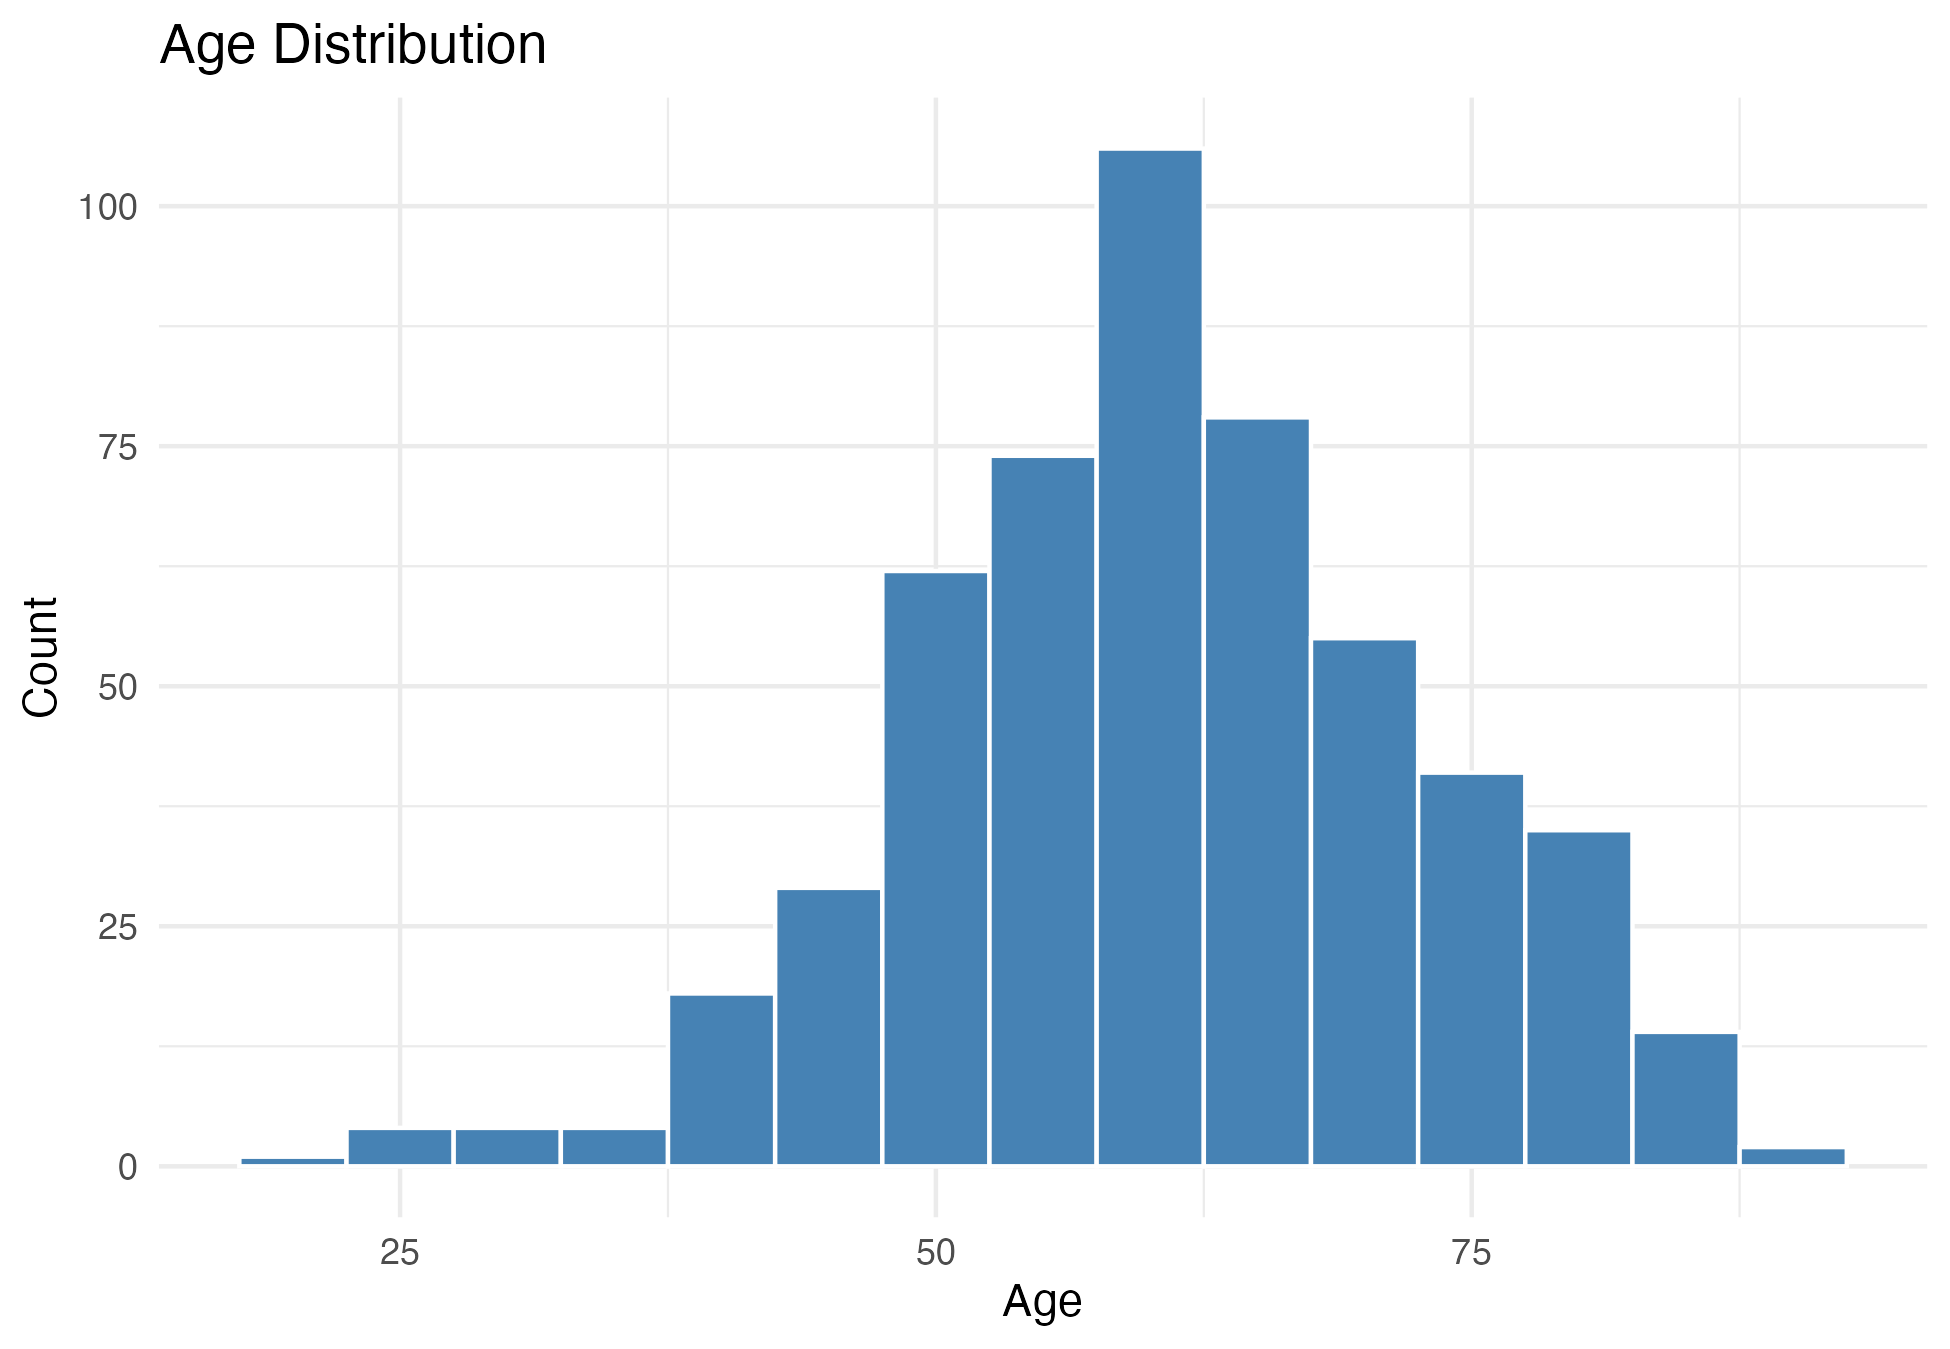
\includegraphics[width=0.8\linewidth]{../outputs/plots/eda/eda_age_distribution}

\paragraph{Gender distribution}\label{gender-distribution}

\begin{Shaded}
\begin{Highlighting}[]
\NormalTok{knitr}\SpecialCharTok{::}\FunctionTok{include\_graphics}\NormalTok{(}\FunctionTok{here}\NormalTok{(}\StringTok{"outputs"}\NormalTok{, }\StringTok{"plots"}\NormalTok{, }\StringTok{"eda"}\NormalTok{, }\StringTok{"eda\_gender\_distribution.png"}\NormalTok{))}
\end{Highlighting}
\end{Shaded}

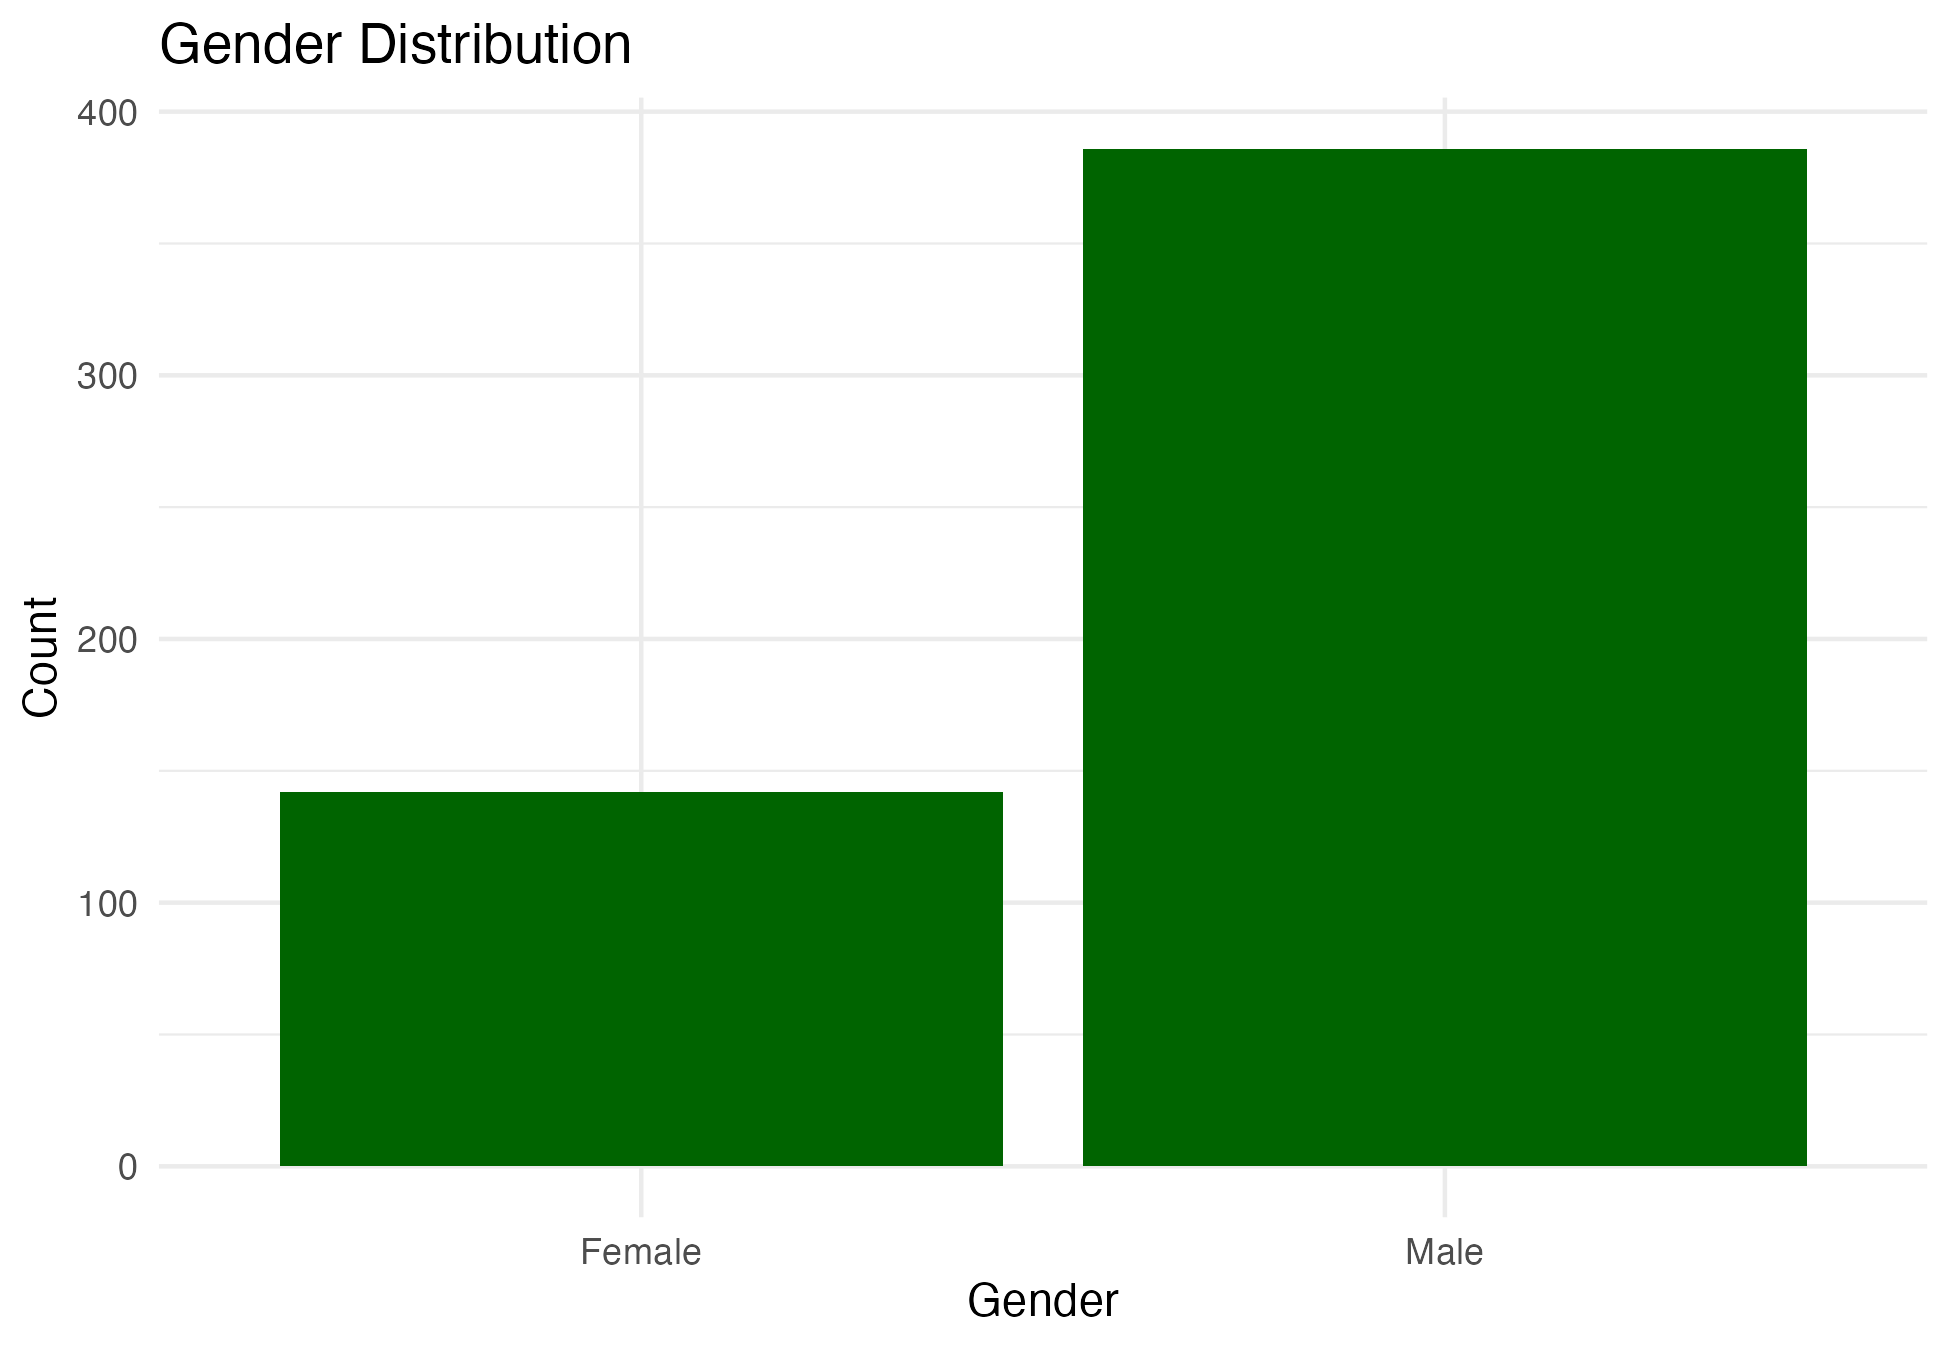
\includegraphics[width=0.8\linewidth]{../outputs/plots/eda/eda_gender_distribution}

\paragraph{Tumor stage counts}\label{tumor-stage-counts}

\begin{Shaded}
\begin{Highlighting}[]
\NormalTok{knitr}\SpecialCharTok{::}\FunctionTok{include\_graphics}\NormalTok{(}\FunctionTok{here}\NormalTok{(}\StringTok{"outputs"}\NormalTok{, }\StringTok{"plots"}\NormalTok{, }\StringTok{"eda"}\NormalTok{, }\StringTok{"eda\_stage\_distribution.png"}\NormalTok{))}
\end{Highlighting}
\end{Shaded}

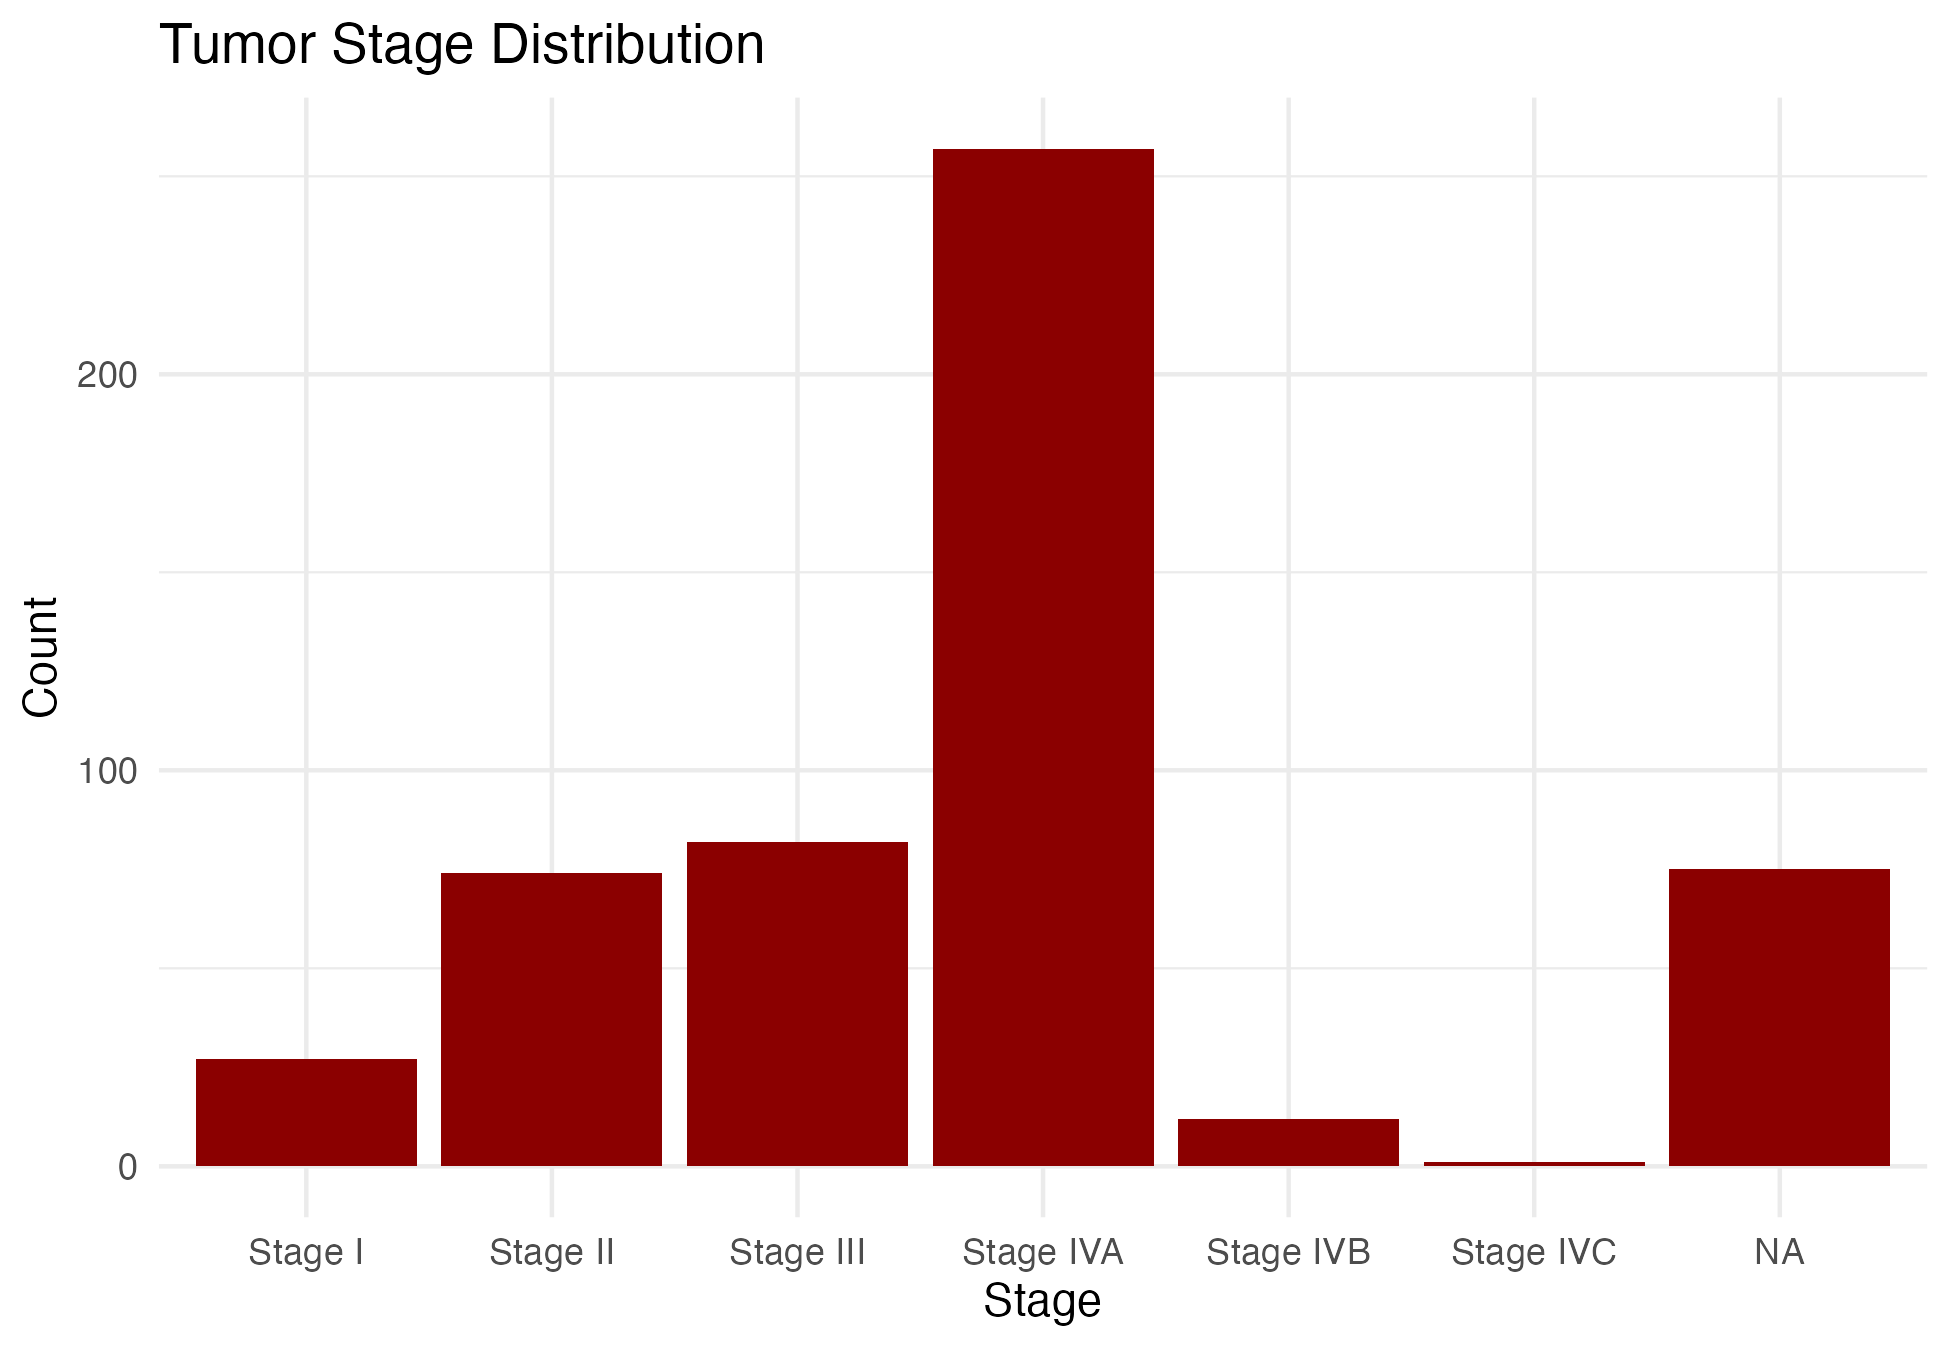
\includegraphics[width=0.8\linewidth]{../outputs/plots/eda/eda_stage_distribution}

\paragraph{Survival time distribution}\label{survival-time-distribution}

\begin{Shaded}
\begin{Highlighting}[]
\NormalTok{knitr}\SpecialCharTok{::}\FunctionTok{include\_graphics}\NormalTok{(}\FunctionTok{here}\NormalTok{(}\StringTok{"outputs"}\NormalTok{, }\StringTok{"plots"}\NormalTok{, }\StringTok{"eda"}\NormalTok{, }\StringTok{"eda\_os\_distribution.png"}\NormalTok{))}
\end{Highlighting}
\end{Shaded}

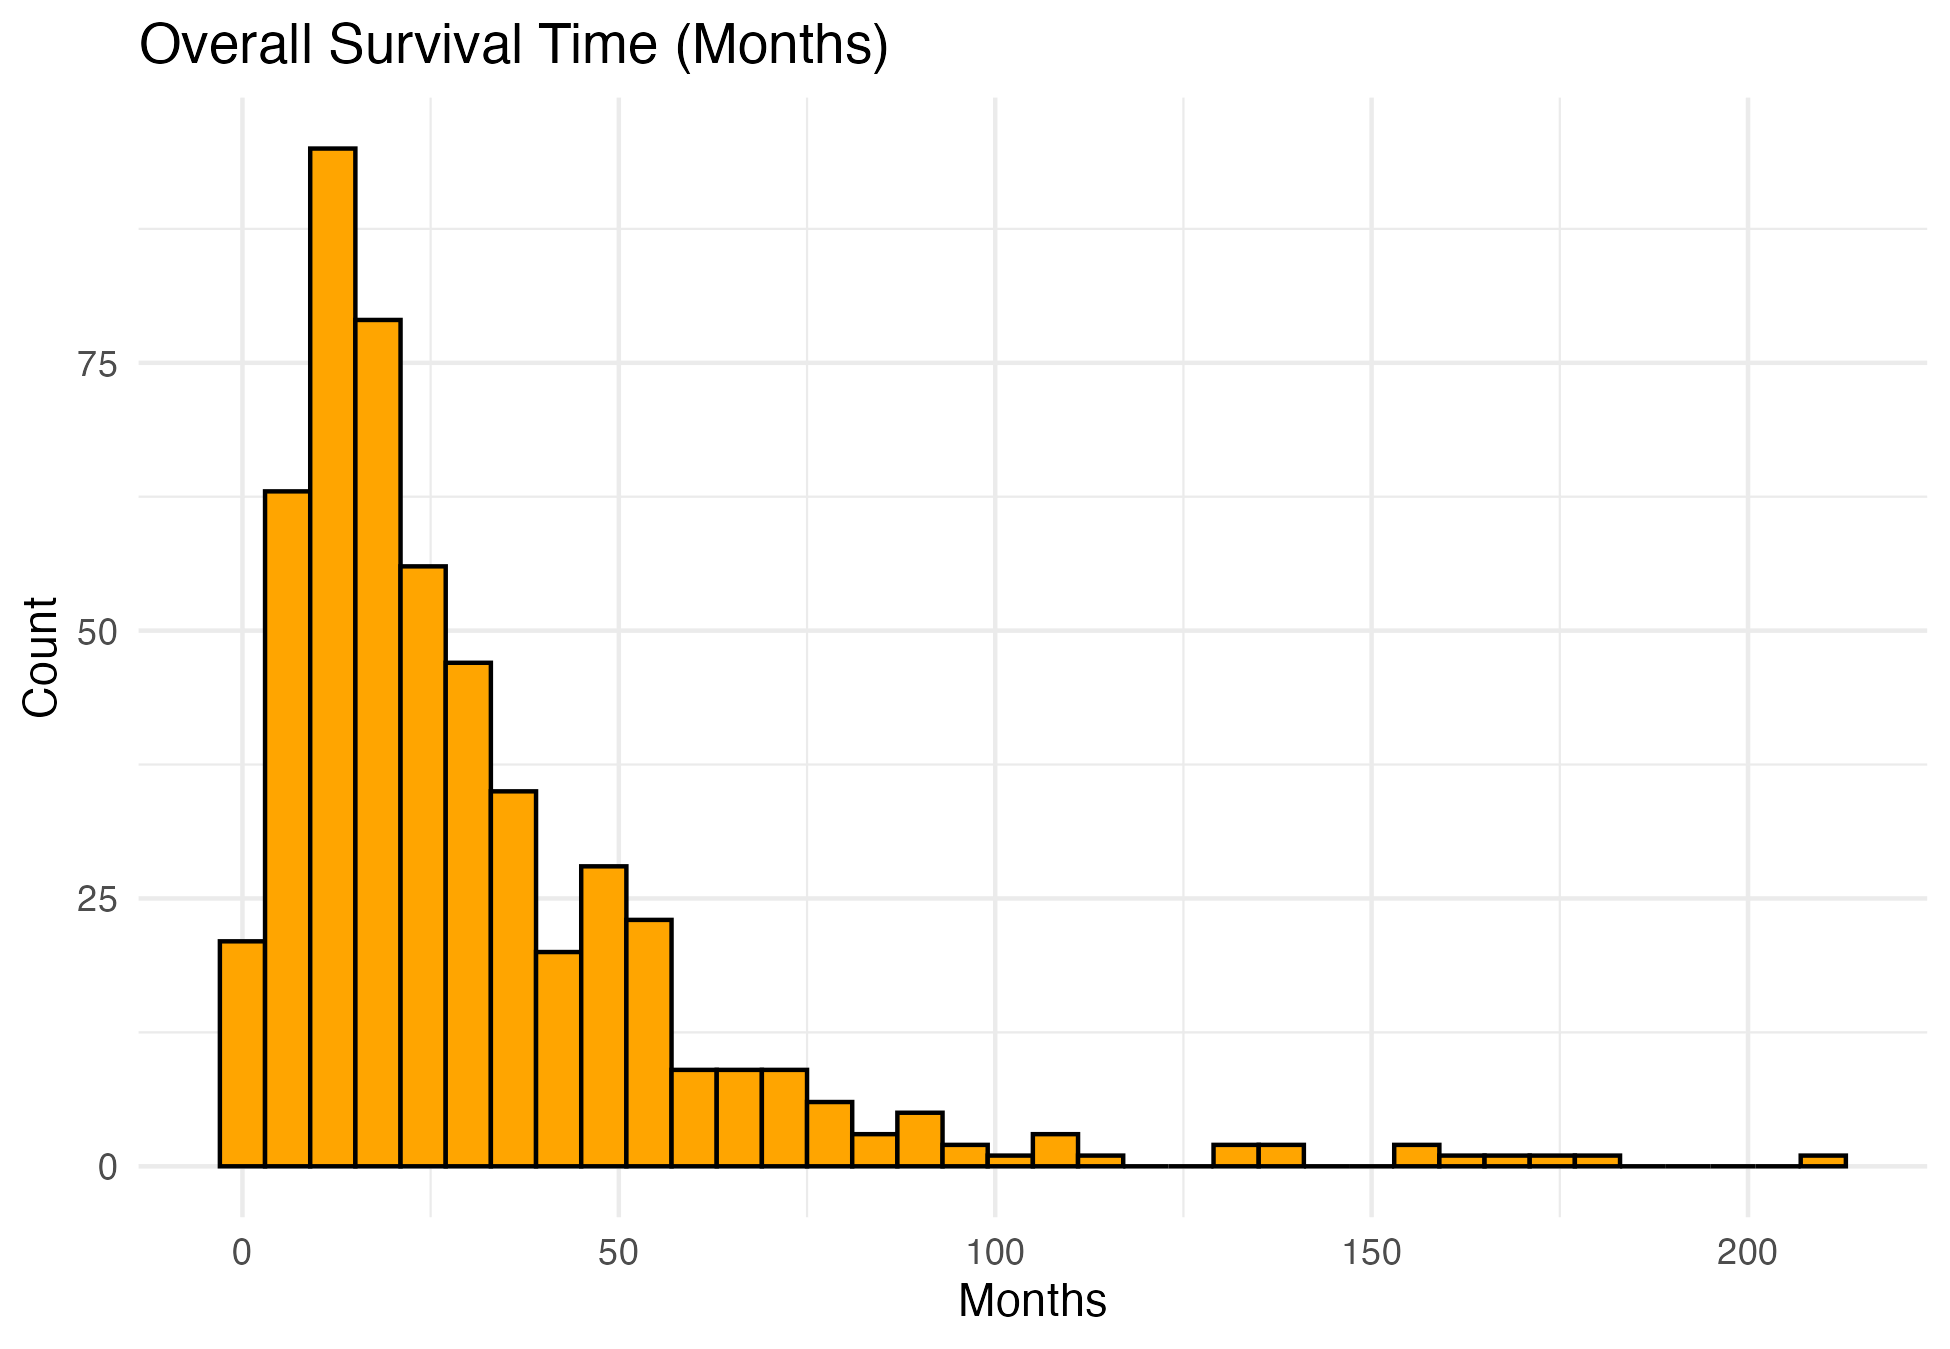
\includegraphics[width=0.8\linewidth]{../outputs/plots/eda/eda_os_distribution}

\section{4. Traditional Survival
Modeling}\label{traditional-survival-modeling}

\subsection{Kaplan-Meier Survival Estimates by
Stage}\label{kaplan-meier-survival-estimates-by-stage}

\begin{Shaded}
\begin{Highlighting}[]
\NormalTok{knitr}\SpecialCharTok{::}\FunctionTok{include\_graphics}\NormalTok{(}\FunctionTok{here}\NormalTok{(}\StringTok{"outputs"}\NormalTok{, }\StringTok{"plots"}\NormalTok{, }\StringTok{"survival"}\NormalTok{, }\StringTok{"km\_survival\_by\_stage.png"}\NormalTok{))}
\end{Highlighting}
\end{Shaded}

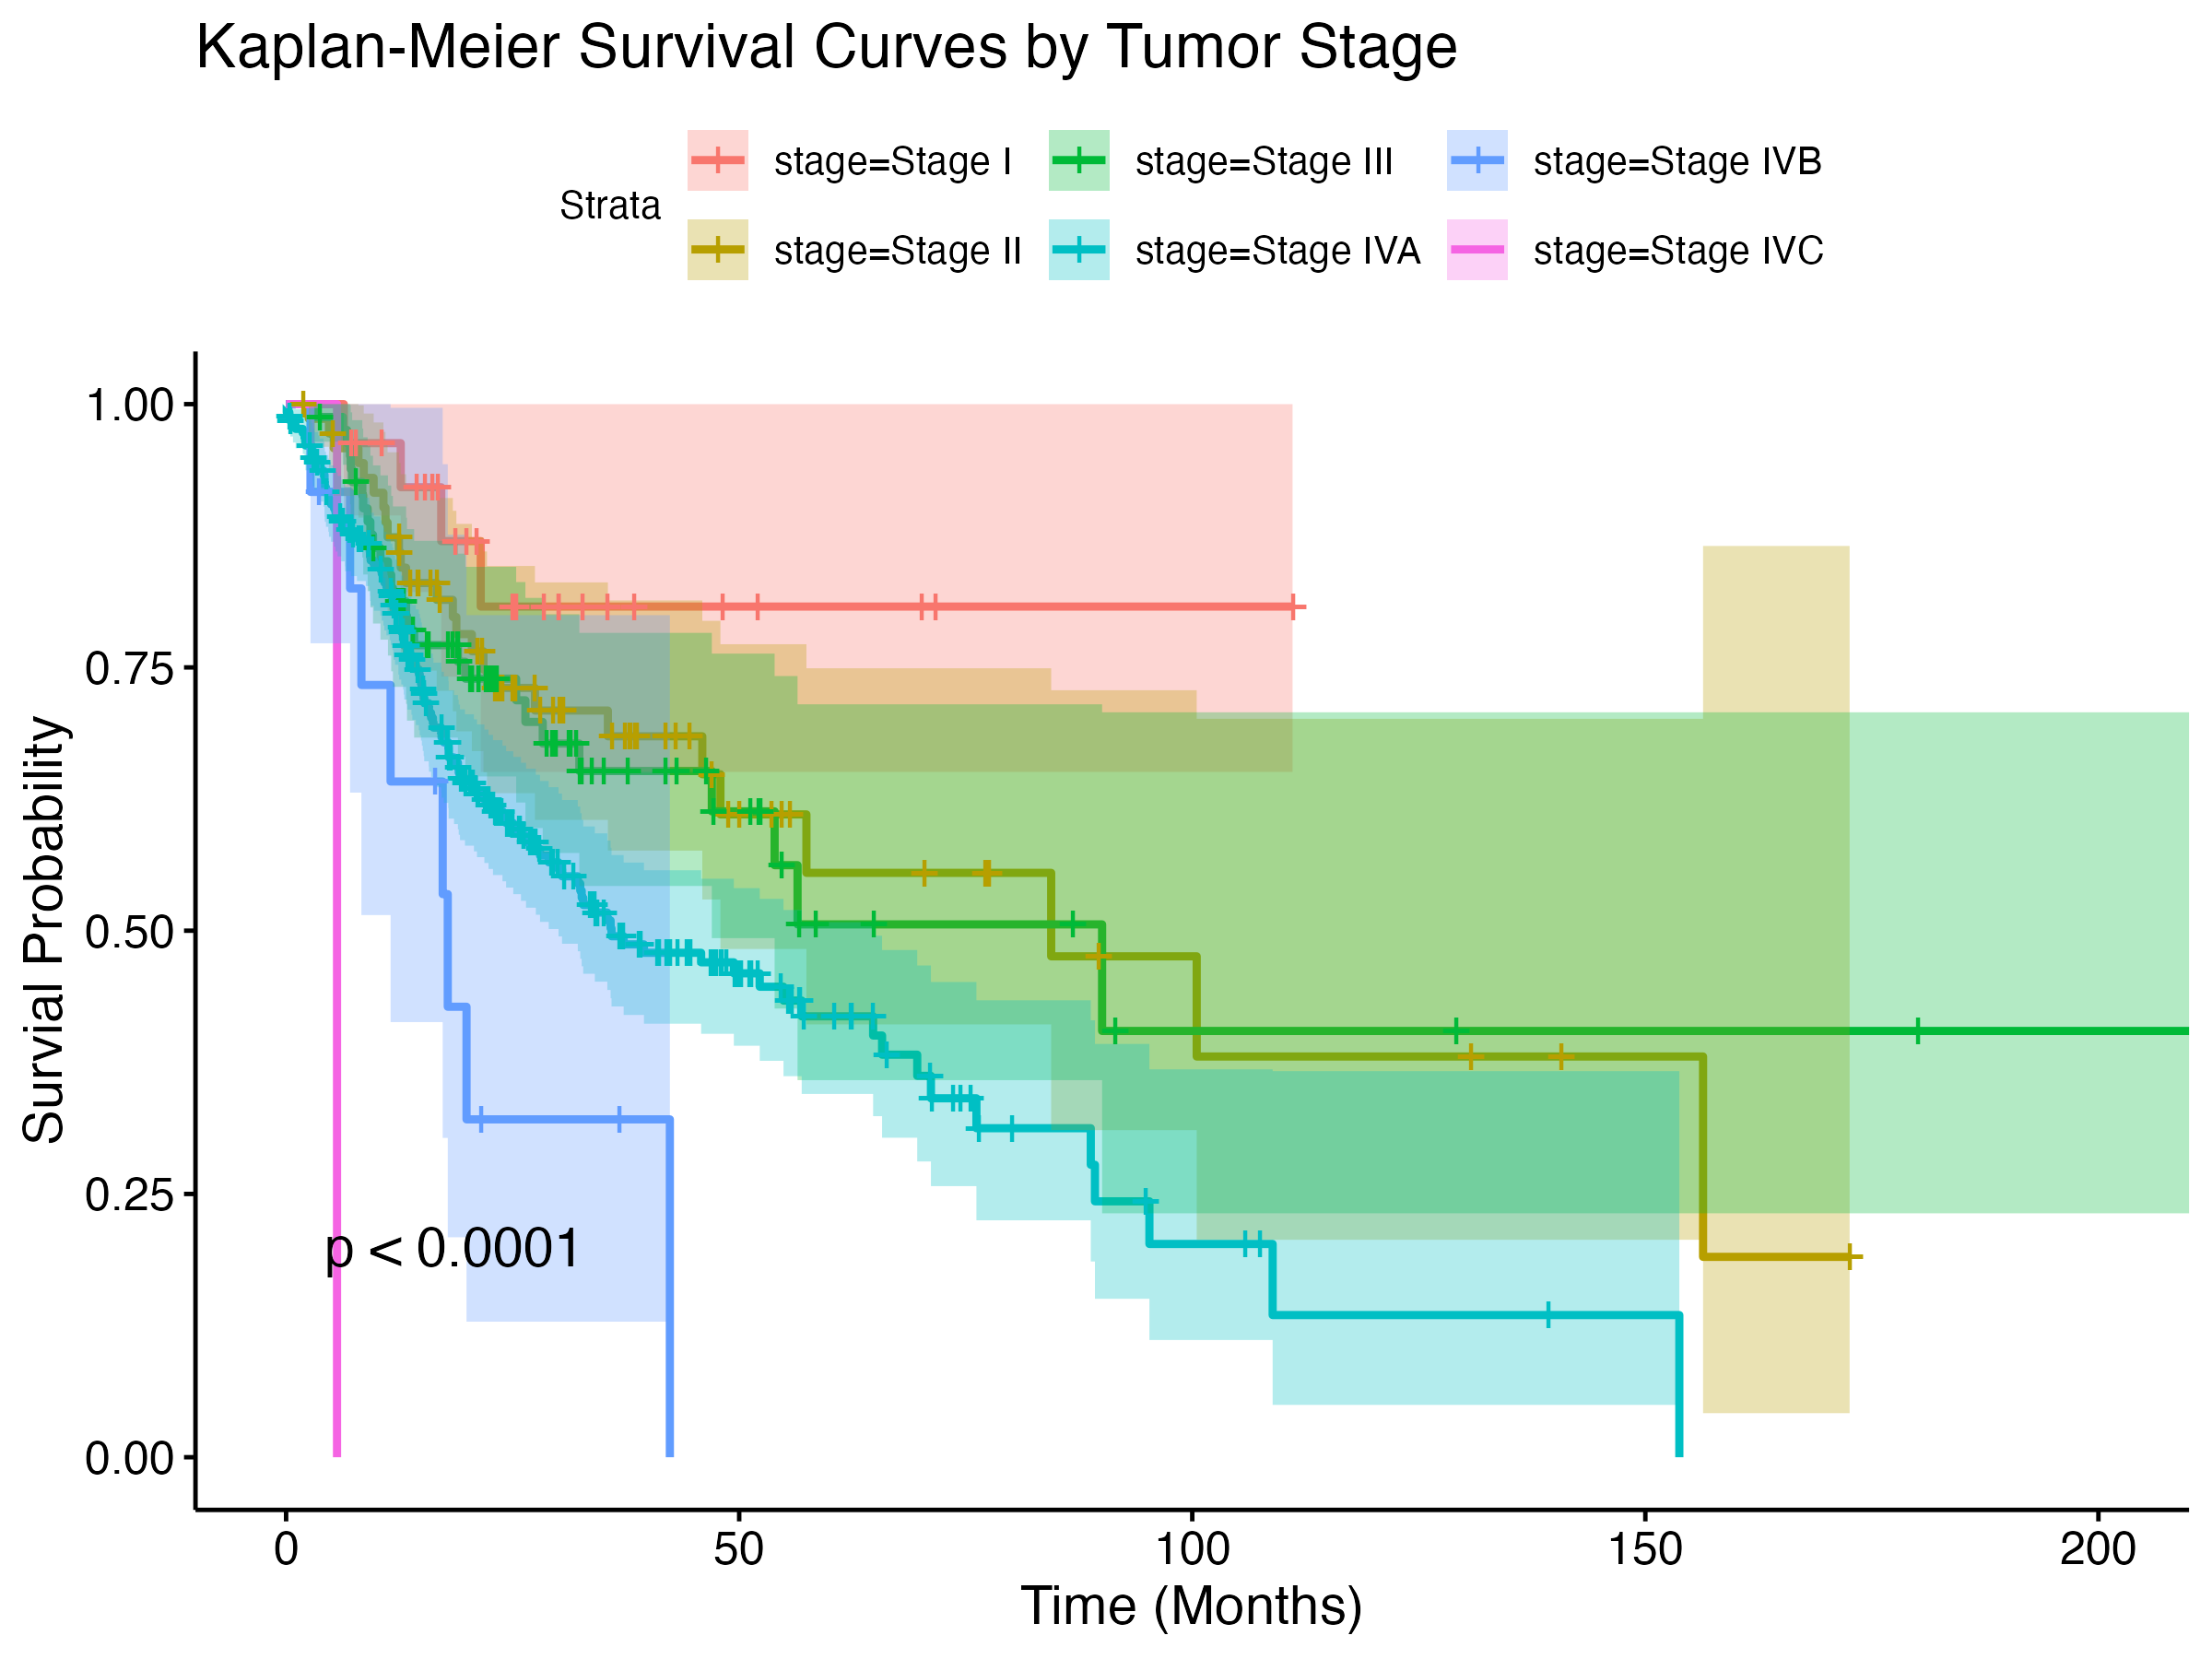
\includegraphics[width=0.8\linewidth]{../outputs/plots/survival/km_survival_by_stage}

\subsection{Kaplan-Meier Survival Estimates by
Gender}\label{kaplan-meier-survival-estimates-by-gender}

\begin{Shaded}
\begin{Highlighting}[]
\NormalTok{knitr}\SpecialCharTok{::}\FunctionTok{include\_graphics}\NormalTok{(}\FunctionTok{here}\NormalTok{(}\StringTok{"outputs"}\NormalTok{, }\StringTok{"plots"}\NormalTok{, }\StringTok{"survival"}\NormalTok{, }\StringTok{"km\_survival\_by\_gender.png"}\NormalTok{))}
\end{Highlighting}
\end{Shaded}

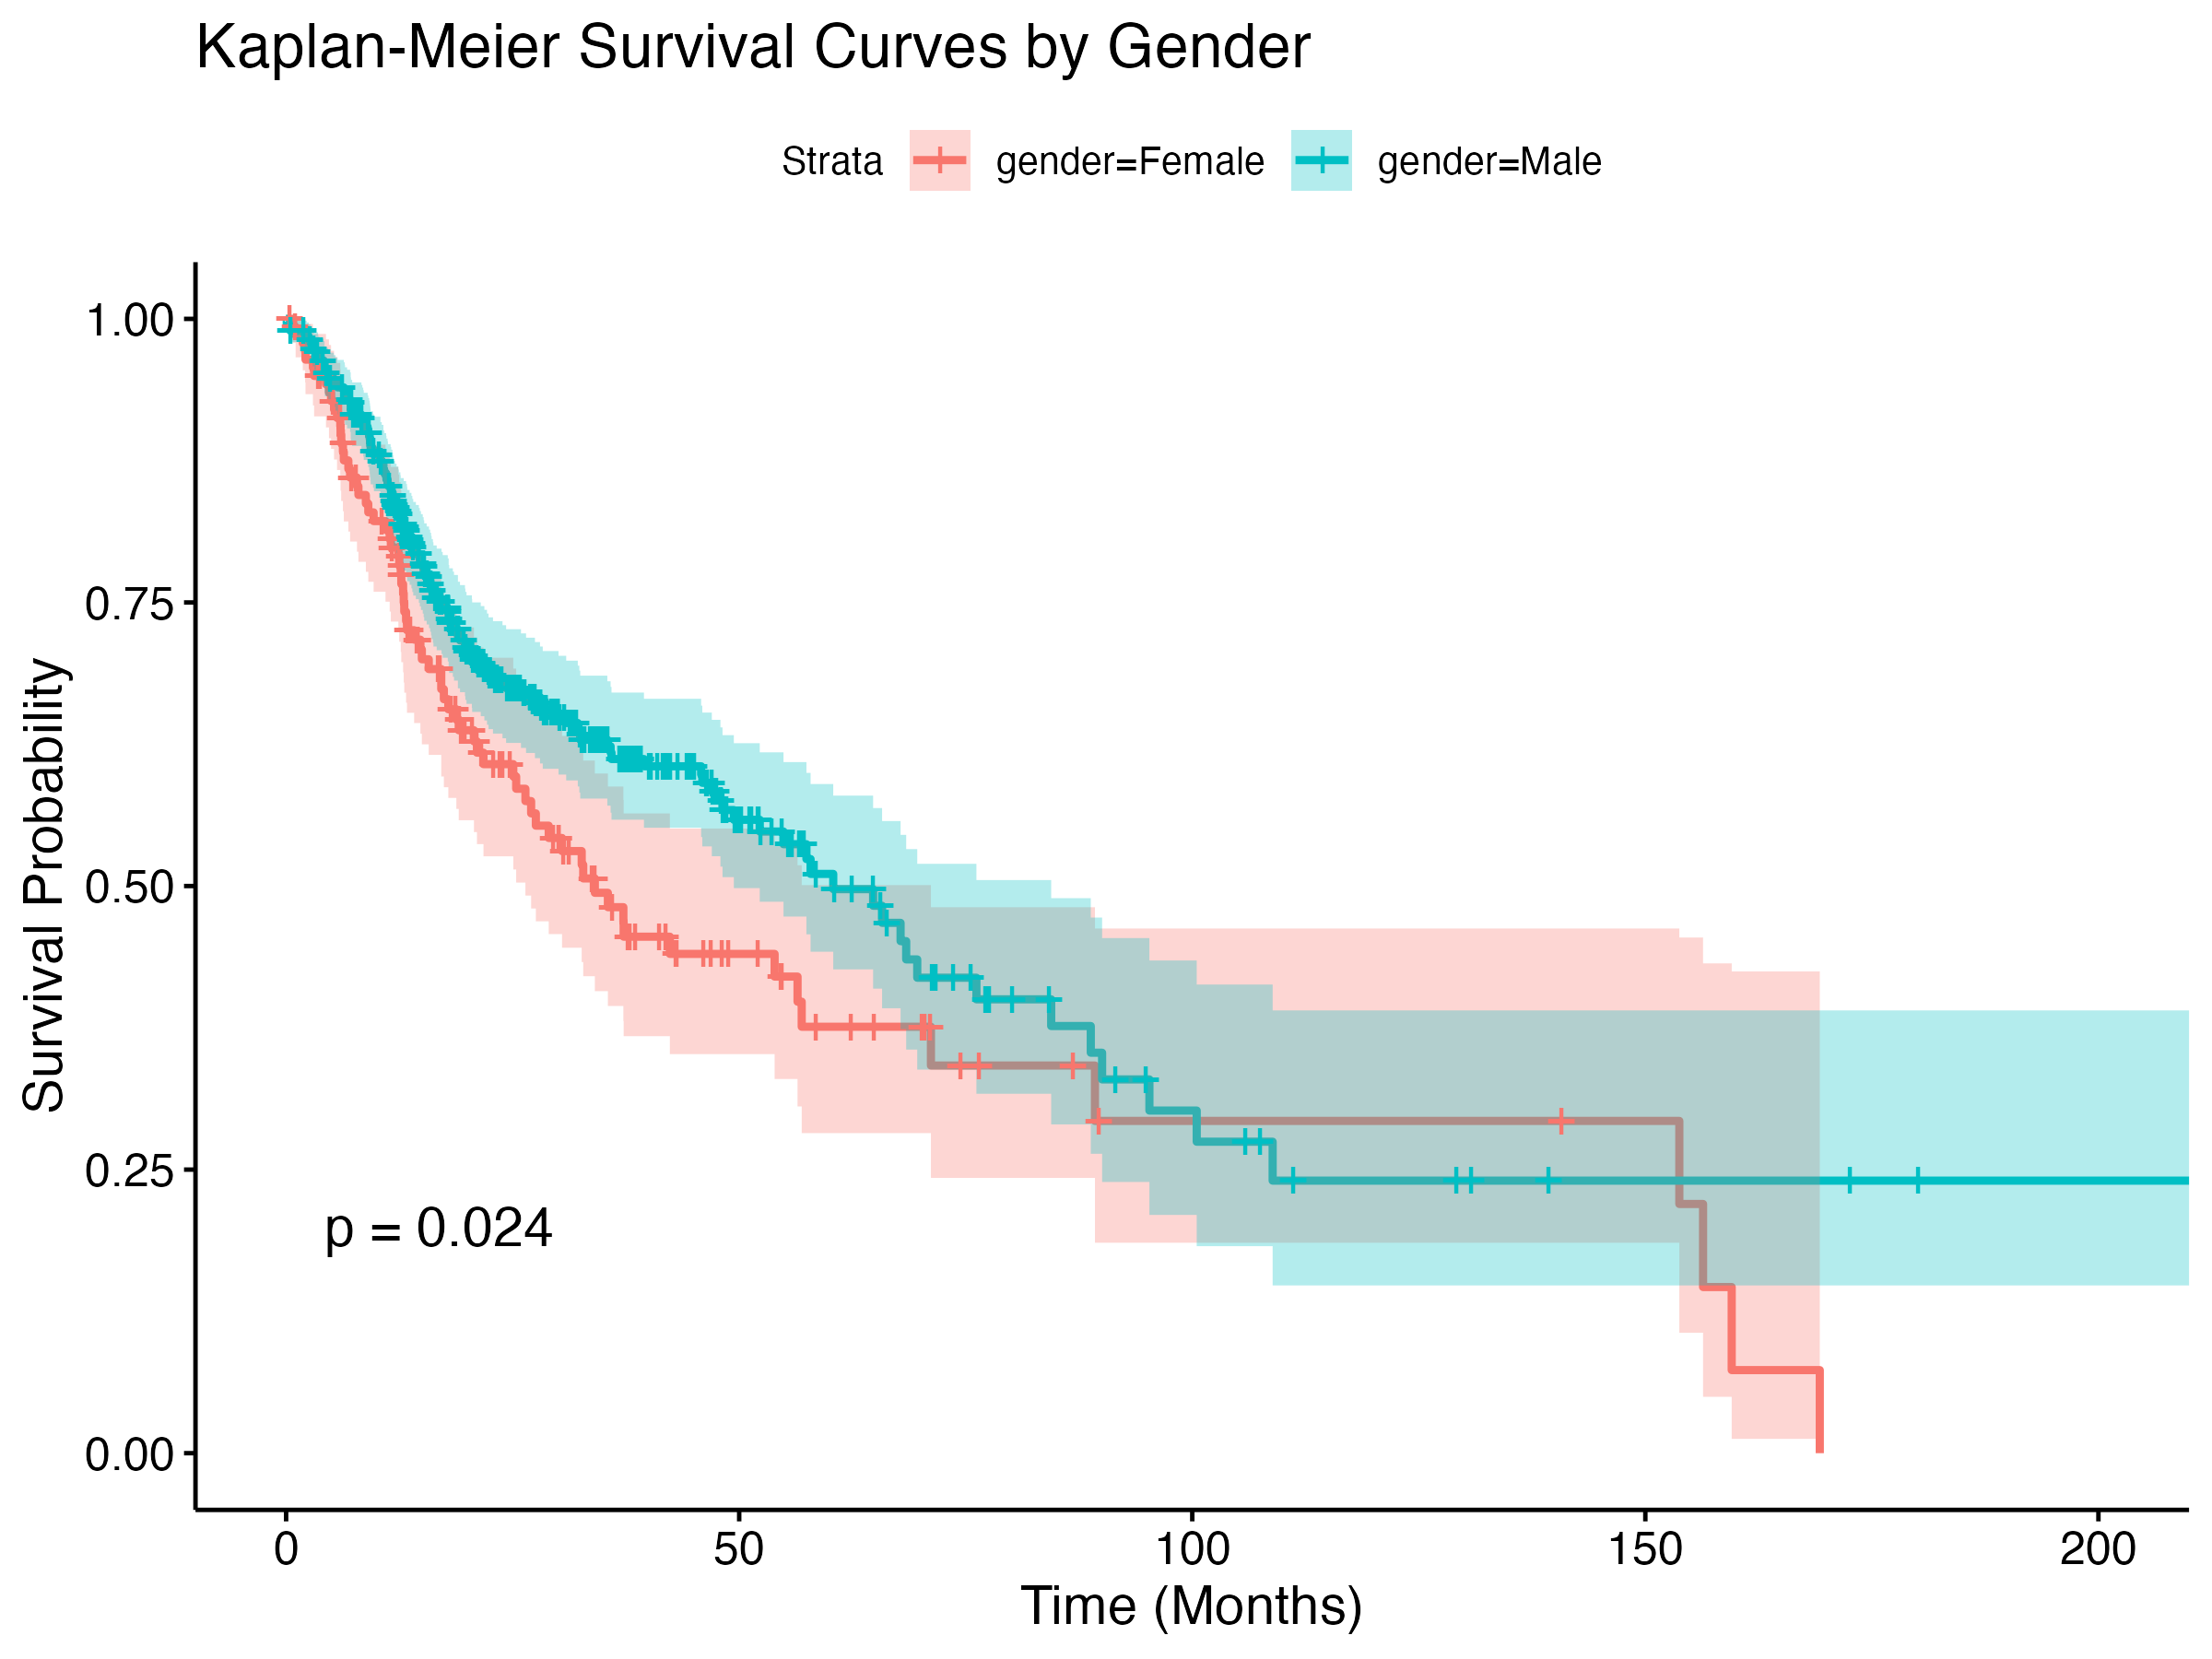
\includegraphics[width=0.8\linewidth]{../outputs/plots/survival/km_survival_by_gender}

\subsection{Cox Proportional Hazards
Model}\label{cox-proportional-hazards-model}

\begin{Shaded}
\begin{Highlighting}[]
\FunctionTok{summary}\NormalTok{(cox\_model)}
\end{Highlighting}
\end{Shaded}

\begin{verbatim}
## Call:
## coxph(formula = surv_object ~ age + gender + stage + primary_site, 
##     data = clinical_data)
## 
##   n= 451, number of events= 192 
##    (77 observations deleted due to missingness)
## 
##                                 coef exp(coef)  se(coef)      z Pr(>|z|)    
## age                         0.024505  1.024808  0.007629  3.212  0.00132 ** 
## genderMale                 -0.101795  0.903214  0.174214 -0.584  0.55901    
## stage.L                     3.157983 23.523099  0.717522  4.401 1.08e-05 ***
## stage.Q                     0.959914  2.611472  0.642036  1.495  0.13489    
## stage.C                     0.710218  2.034435  0.490139  1.449  0.14733    
## stage^4                     0.114849  1.121704  0.339548  0.338  0.73518    
## stage^5                     0.204761  1.227231  0.203219  1.008  0.31365    
## primary_siteBase of tongue  0.492424  1.636278  0.547594  0.899  0.36852    
## primary_siteBuccal Mucosa   0.081714  1.085145  0.526609  0.155  0.87669    
## primary_siteFloor of mouth  0.605504  1.832175  0.422417  1.433  0.15174    
## primary_siteHard Palate    -0.323656  0.723499  0.815856 -0.397  0.69158    
## primary_siteHypopharynx     0.300177  1.350098  0.699257  0.429  0.66772    
## primary_siteLarynx         -0.100142  0.904709  0.421438 -0.238  0.81218    
## primary_siteLip             1.136926  3.117171  1.107896  1.026  0.30480    
## primary_siteOral Cavity     0.461697  1.586764  0.416135  1.109  0.26722    
## primary_siteOral Tongue     0.509655  1.664717  0.417488  1.221  0.22217    
## primary_siteOropharynx      0.874632  2.397993  0.825316  1.060  0.28926    
## primary_siteTonsil         -0.070723  0.931720  0.565551 -0.125  0.90048    
## ---
## Signif. codes:  0 '***' 0.001 '**' 0.01 '*' 0.05 '.' 0.1 ' ' 1
## 
##                            exp(coef) exp(-coef) lower .95 upper .95
## age                           1.0248    0.97579    1.0096     1.040
## genderMale                    0.9032    1.10716    0.6419     1.271
## stage.L                      23.5231    0.04251    5.7642    95.995
## stage.Q                       2.6115    0.38293    0.7420     9.192
## stage.C                       2.0344    0.49154    0.7785     5.317
## stage^4                       1.1217    0.89150    0.5766     2.182
## stage^5                       1.2272    0.81484    0.8240     1.828
## primary_siteBase of tongue    1.6363    0.61114    0.5594     4.786
## primary_siteBuccal Mucosa     1.0851    0.92154    0.3866     3.046
## primary_siteFloor of mouth    1.8322    0.54580    0.8006     4.193
## primary_siteHard Palate       0.7235    1.38217    0.1462     3.580
## primary_siteHypopharynx       1.3501    0.74069    0.3429     5.316
## primary_siteLarynx            0.9047    1.10533    0.3961     2.067
## primary_siteLip               3.1172    0.32080    0.3554    27.340
## primary_siteOral Cavity       1.5868    0.63021    0.7019     3.587
## primary_siteOral Tongue       1.6647    0.60070    0.7345     3.773
## primary_siteOropharynx        2.3980    0.41702    0.4757    12.088
## primary_siteTonsil            0.9317    1.07328    0.3075     2.823
## 
## Concordance= 0.646  (se = 0.023 )
## Likelihood ratio test= 53.42  on 18 df,   p=2e-05
## Wald test            = 54.38  on 18 df,   p=2e-05
## Score (logrank) test = 61.31  on 18 df,   p=1e-06
\end{verbatim}

\section{5. Machine Learning Models (Binary
Classification)}\label{machine-learning-models-binary-classification}

We defined a binary outcome: survival beyond 24 months.

\subsection{Random Forest}\label{random-forest}

\begin{Shaded}
\begin{Highlighting}[]
\FunctionTok{print}\NormalTok{(rf\_model\_cv)}
\end{Highlighting}
\end{Shaded}

\begin{verbatim}
## Random Forest 
## 
## 451 samples
##   4 predictor
##   2 classes: 'Not_Survived', 'Survived' 
## 
## Pre-processing: centered (18), scaled (18) 
## Resampling: Cross-Validated (10 fold) 
## Summary of sample sizes: 405, 405, 407, 407, 405, 406, ... 
## Resampling results across tuning parameters:
## 
##   mtry  ROC        Sens       Spec     
##    2    0.5563022  0.8392308  0.1786842
##   10    0.5081213  0.6200000  0.3923684
##   18    0.5146632  0.6435385  0.3823684
## 
## ROC was used to select the optimal model using the largest value.
## The final value used for the model was mtry = 2.
\end{verbatim}

\begin{Shaded}
\begin{Highlighting}[]
\NormalTok{knitr}\SpecialCharTok{::}\FunctionTok{include\_graphics}\NormalTok{(}\FunctionTok{here}\NormalTok{(}\StringTok{"outputs"}\NormalTok{, }\StringTok{"plots"}\NormalTok{, }\StringTok{"ml"}\NormalTok{, }\StringTok{"rf\_cv\_roc\_curve.png"}\NormalTok{))}
\end{Highlighting}
\end{Shaded}

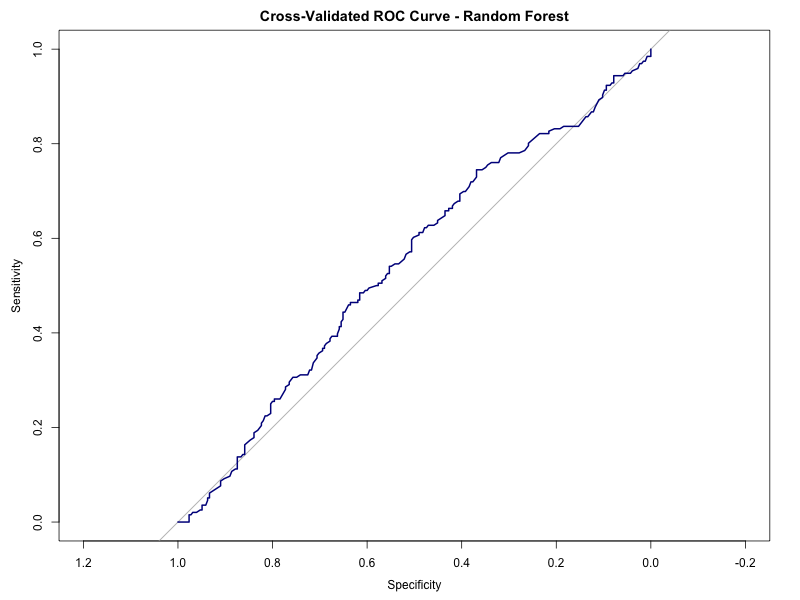
\includegraphics[width=0.8\linewidth]{../outputs/plots/ml/rf_cv_roc_curve}

\subsection{Logistic Regression with L1
Regularization}\label{logistic-regression-with-l1-regularization}

\begin{Shaded}
\begin{Highlighting}[]
\FunctionTok{print}\NormalTok{(logistic\_model)}
\end{Highlighting}
\end{Shaded}

\begin{verbatim}
## glmnet 
## 
## 451 samples
##   5 predictor
##   2 classes: 'Not_Survived', 'Survived' 
## 
## Pre-processing: centered (14), scaled (14) 
## Resampling: Cross-Validated (10 fold) 
## Summary of sample sizes: 405, 405, 407, 407, 405, 406, ... 
## Resampling results across tuning parameters:
## 
##   alpha  lambda        ROC        Sens       Spec     
##   0.10   0.0001061109  0.5825927  0.7730769  0.3102632
##   0.10   0.0010611095  0.5825927  0.7730769  0.3155263
##   0.10   0.0106110950  0.5832717  0.7884615  0.3055263
##   0.55   0.0001061109  0.5822004  0.7769231  0.3155263
##   0.55   0.0010611095  0.5828211  0.7769231  0.3155263
##   0.55   0.0106110950  0.5825275  0.8001538  0.2955263
##   1.00   0.0001061109  0.5819899  0.7769231  0.3155263
##   1.00   0.0010611095  0.5832211  0.7807692  0.3105263
##   1.00   0.0106110950  0.5875901  0.8158462  0.2605263
## 
## ROC was used to select the optimal model using the largest value.
## The final values used for the model were alpha = 1 and lambda = 0.01061109.
\end{verbatim}

\begin{Shaded}
\begin{Highlighting}[]
\NormalTok{knitr}\SpecialCharTok{::}\FunctionTok{include\_graphics}\NormalTok{(}\FunctionTok{here}\NormalTok{(}\StringTok{"outputs"}\NormalTok{, }\StringTok{"plots"}\NormalTok{, }\StringTok{"ml"}\NormalTok{, }\StringTok{"logistic\_roc\_curve.png"}\NormalTok{))}
\end{Highlighting}
\end{Shaded}

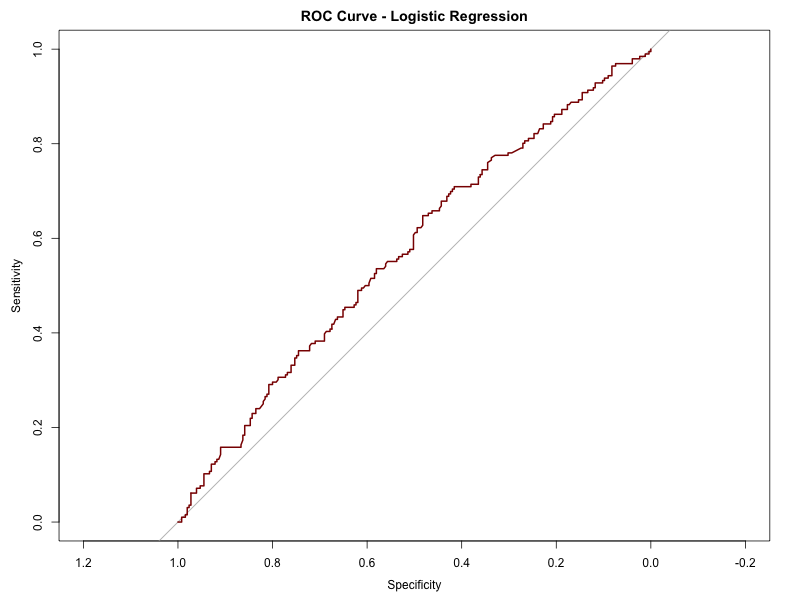
\includegraphics[width=0.8\linewidth]{../outputs/plots/ml/logistic_roc_curve}

\subsection{XGBoost}\label{xgboost}

\begin{Shaded}
\begin{Highlighting}[]
\FunctionTok{print}\NormalTok{(xgb\_model)}
\end{Highlighting}
\end{Shaded}

\begin{verbatim}
## eXtreme Gradient Boosting 
## 
## 451 samples
##   5 predictor
##   2 classes: 'Not_Survived', 'Survived' 
## 
## Pre-processing: centered (14), scaled (14) 
## Resampling: Cross-Validated (10 fold) 
## Summary of sample sizes: 406, 406, 407, 405, 406, 407, ... 
## Resampling results across tuning parameters:
## 
##   eta  max_depth  colsample_bytree  subsample  nrounds  ROC        Sens     
##   0.3  1          0.6               0.50        50      0.5158919  0.7404615
##   0.3  1          0.6               0.50       100      0.5143684  0.7332308
##   0.3  1          0.6               0.50       150      0.5369804  0.7321538
##   0.3  1          0.6               0.75        50      0.5323233  0.7878462
##   0.3  1          0.6               0.75       100      0.5400812  0.6972308
##   0.3  1          0.6               0.75       150      0.5208741  0.6655385
##   0.3  1          0.6               1.00        50      0.5511336  0.7921538
##   0.3  1          0.6               1.00       100      0.5409709  0.7484615
##   0.3  1          0.6               1.00       150      0.5372893  0.7090769
##   0.3  1          0.8               0.50        50      0.5264727  0.7253846
##   0.3  1          0.8               0.50       100      0.5213160  0.6896923
##   0.3  1          0.8               0.50       150      0.5233826  0.7090769
##   0.3  1          0.8               0.75        50      0.5502684  0.7373846
##   0.3  1          0.8               0.75       100      0.5315957  0.7012308
##   0.3  1          0.8               0.75       150      0.5429352  0.7130769
##   0.3  1          0.8               1.00        50      0.5431504  0.7920000
##   0.3  1          0.8               1.00       100      0.5375796  0.7484615
##   0.3  1          0.8               1.00       150      0.5332164  0.7250769
##   0.3  2          0.6               0.50        50      0.5032947  0.6581538
##   0.3  2          0.6               0.50       100      0.5323018  0.6616923
##   0.3  2          0.6               0.50       150      0.5394480  0.6386154
##   0.3  2          0.6               0.75        50      0.5157820  0.6780000
##   0.3  2          0.6               0.75       100      0.5121053  0.6621538
##   0.3  2          0.6               0.75       150      0.5316968  0.6384615
##   0.3  2          0.6               1.00        50      0.5616087  0.7130769
##   0.3  2          0.6               1.00       100      0.5616957  0.7049231
##   0.3  2          0.6               1.00       150      0.5563555  0.6653846
##   0.3  2          0.8               0.50        50      0.5316800  0.6858462
##   0.3  2          0.8               0.50       100      0.5397466  0.6698462
##   0.3  2          0.8               0.50       150      0.5359146  0.6503077
##   0.3  2          0.8               0.75        50      0.5344302  0.7006154
##   0.3  2          0.8               0.75       100      0.5431247  0.6573846
##   0.3  2          0.8               0.75       150      0.5381943  0.6421538
##   0.3  2          0.8               1.00        50      0.5494257  0.7053846
##   0.3  2          0.8               1.00       100      0.5378466  0.6693846
##   0.3  2          0.8               1.00       150      0.5379941  0.6578462
##   0.3  3          0.6               0.50        50      0.5180630  0.6540000
##   0.3  3          0.6               0.50       100      0.5076306  0.6229231
##   0.3  3          0.6               0.50       150      0.5051073  0.6107692
##   0.3  3          0.6               0.75        50      0.5109223  0.6698462
##   0.3  3          0.6               0.75       100      0.5187275  0.6423077
##   0.3  3          0.6               0.75       150      0.5204182  0.6229231
##   0.3  3          0.6               1.00        50      0.5385978  0.6770769
##   0.3  3          0.6               1.00       100      0.5342366  0.6381538
##   0.3  3          0.6               1.00       150      0.5285200  0.6263077
##   0.3  3          0.8               0.50        50      0.5252656  0.6075385
##   0.3  3          0.8               0.50       100      0.5099405  0.6112308
##   0.3  3          0.8               0.50       150      0.5133235  0.6038462
##   0.3  3          0.8               0.75        50      0.5223437  0.6266154
##   0.3  3          0.8               0.75       100      0.5093004  0.5916923
##   0.3  3          0.8               0.75       150      0.5090814  0.6000000
##   0.3  3          0.8               1.00        50      0.5384006  0.6623077
##   0.3  3          0.8               1.00       100      0.5370897  0.6149231
##   0.3  3          0.8               1.00       150      0.5308405  0.5836923
##   0.4  1          0.6               0.50        50      0.5465743  0.7410769
##   0.4  1          0.6               0.50       100      0.5263457  0.7013846
##   0.4  1          0.6               0.50       150      0.5343968  0.7049231
##   0.4  1          0.6               0.75        50      0.5460915  0.7204615
##   0.4  1          0.6               0.75       100      0.5425411  0.7098462
##   0.4  1          0.6               0.75       150      0.5381265  0.7086154
##   0.4  1          0.6               1.00        50      0.5442358  0.7718462
##   0.4  1          0.6               1.00       100      0.5345796  0.7207692
##   0.4  1          0.6               1.00       150      0.5348603  0.7052308
##   0.4  1          0.8               0.50        50      0.5238769  0.7253846
##   0.4  1          0.8               0.50       100      0.5067982  0.6935385
##   0.4  1          0.8               0.50       150      0.5348466  0.6892308
##   0.4  1          0.8               0.75        50      0.5499737  0.7481538
##   0.4  1          0.8               0.75       100      0.5344506  0.7204615
##   0.4  1          0.8               0.75       150      0.5360318  0.6847692
##   0.4  1          0.8               1.00        50      0.5400217  0.7764615
##   0.4  1          0.8               1.00       100      0.5359812  0.7172308
##   0.4  1          0.8               1.00       150      0.5302387  0.7016923
##   0.4  2          0.6               0.50        50      0.5452771  0.6901538
##   0.4  2          0.6               0.50       100      0.5324346  0.6181538
##   0.4  2          0.6               0.50       150      0.5092053  0.5984615
##   0.4  2          0.6               0.75        50      0.5291251  0.6849231
##   0.4  2          0.6               0.75       100      0.5156227  0.6621538
##   0.4  2          0.6               0.75       150      0.5191953  0.6309231
##   0.4  2          0.6               1.00        50      0.5507682  0.6855385
##   0.4  2          0.6               1.00       100      0.5465504  0.6500000
##   0.4  2          0.6               1.00       150      0.5462196  0.6458462
##   0.4  2          0.8               0.50        50      0.5608255  0.6896923
##   0.4  2          0.8               0.50       100      0.5437200  0.6544615
##   0.4  2          0.8               0.50       150      0.5304868  0.6307692
##   0.4  2          0.8               0.75        50      0.5212571  0.6536923
##   0.4  2          0.8               0.75       100      0.5157538  0.6307692
##   0.4  2          0.8               0.75       150      0.5249559  0.6263077
##   0.4  2          0.8               1.00        50      0.5391719  0.6775385
##   0.4  2          0.8               1.00       100      0.5436132  0.6496923
##   0.4  2          0.8               1.00       150      0.5436087  0.6378462
##   0.4  3          0.6               0.50        50      0.5026818  0.6387692
##   0.4  3          0.6               0.50       100      0.4879356  0.6001538
##   0.4  3          0.6               0.50       150      0.5000101  0.6158462
##   0.4  3          0.6               0.75        50      0.5211451  0.6230769
##   0.4  3          0.6               0.75       100      0.5246162  0.6230769
##   0.4  3          0.6               0.75       150      0.5217130  0.5918462
##   0.4  3          0.6               1.00        50      0.5436261  0.6495385
##   0.4  3          0.6               1.00       100      0.5201808  0.6223077
##   0.4  3          0.6               1.00       150      0.5144255  0.5993846
##   0.4  3          0.8               0.50        50      0.5316806  0.6233846
##   0.4  3          0.8               0.50       100      0.5160283  0.6275385
##   0.4  3          0.8               0.50       150      0.5151583  0.5767692
##   0.4  3          0.8               0.75        50      0.5096138  0.5990769
##   0.4  3          0.8               0.75       100      0.5031951  0.5960000
##   0.4  3          0.8               0.75       150      0.4969227  0.5724615
##   0.4  3          0.8               1.00        50      0.5306615  0.5952308
##   0.4  3          0.8               1.00       100      0.5141551  0.5838462
##   0.4  3          0.8               1.00       150      0.5133457  0.5840000
##   Spec     
##   0.3102632
##   0.2957895
##   0.3405263
##   0.2847368
##   0.3413158
##   0.3457895
##   0.2744737
##   0.3002632
##   0.3257895
##   0.2900000
##   0.3157895
##   0.3257895
##   0.2994737
##   0.3210526
##   0.3521053
##   0.2494737
##   0.2800000
##   0.3157895
##   0.3157895
##   0.3778947
##   0.3926316
##   0.3507895
##   0.3560526
##   0.3713158
##   0.3565789
##   0.3926316
##   0.3923684
##   0.3868421
##   0.3565789
##   0.3768421
##   0.3518421
##   0.3778947
##   0.4139474
##   0.3413158
##   0.3663158
##   0.3865789
##   0.4139474
##   0.4031579
##   0.4086842
##   0.3363158
##   0.3936842
##   0.4184211
##   0.3928947
##   0.4136842
##   0.4294737
##   0.3965789
##   0.3976316
##   0.4289474
##   0.4086842
##   0.4086842
##   0.4442105
##   0.4028947
##   0.4342105
##   0.4492105
##   0.3210526
##   0.3215789
##   0.3207895
##   0.3102632
##   0.3618421
##   0.3621053
##   0.2697368
##   0.3263158
##   0.3263158
##   0.2992105
##   0.3260526
##   0.3660526
##   0.2960526
##   0.3360526
##   0.3465789
##   0.2700000
##   0.3257895
##   0.3307895
##   0.4189474
##   0.4234211
##   0.4392105
##   0.3721053
##   0.3721053
##   0.3823684
##   0.3457895
##   0.3818421
##   0.4126316
##   0.4084211
##   0.4336842
##   0.4236842
##   0.3463158
##   0.3968421
##   0.4126316
##   0.3460526
##   0.3860526
##   0.4065789
##   0.3828947
##   0.3871053
##   0.4131579
##   0.3931579
##   0.4594737
##   0.4494737
##   0.3976316
##   0.4286842
##   0.4450000
##   0.4131579
##   0.4026316
##   0.4184211
##   0.4086842
##   0.4544737
##   0.4342105
##   0.4073684
##   0.4389474
##   0.4292105
## 
## Tuning parameter 'gamma' was held constant at a value of 0
## Tuning
##  parameter 'min_child_weight' was held constant at a value of 1
## ROC was used to select the optimal model using the largest value.
## The final values used for the model were nrounds = 100, max_depth = 2, eta
##  = 0.3, gamma = 0, colsample_bytree = 0.6, min_child_weight = 1 and subsample
##  = 1.
\end{verbatim}

\begin{Shaded}
\begin{Highlighting}[]
\NormalTok{knitr}\SpecialCharTok{::}\FunctionTok{include\_graphics}\NormalTok{(}\FunctionTok{here}\NormalTok{(}\StringTok{"outputs"}\NormalTok{, }\StringTok{"plots"}\NormalTok{, }\StringTok{"ml"}\NormalTok{, }\StringTok{"xgb\_roc\_curve.png"}\NormalTok{))}
\end{Highlighting}
\end{Shaded}

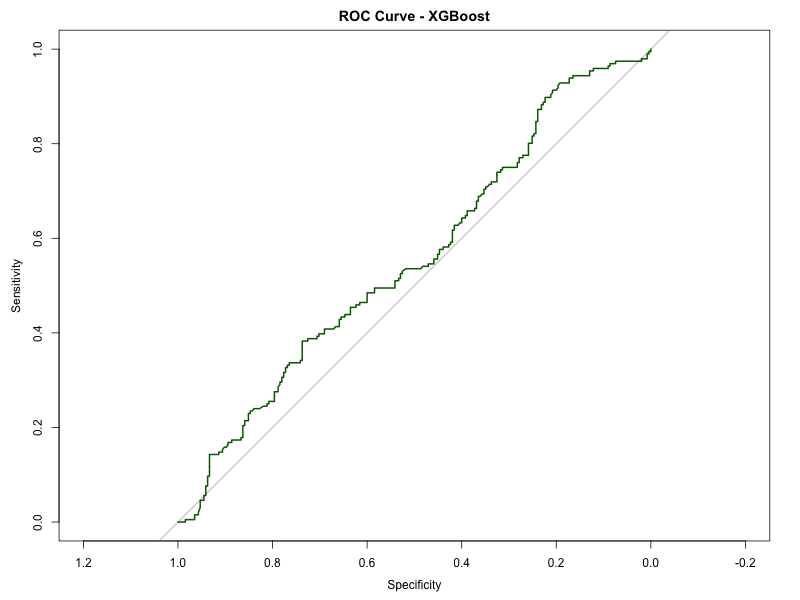
\includegraphics[width=0.8\linewidth]{../outputs/plots/ml/xgb_roc_curve}

\section{6. Time-to-Event Machine Learning
Models}\label{time-to-event-machine-learning-models}

\subsection{Random Survival Forest
(RSF)}\label{random-survival-forest-rsf}

\begin{Shaded}
\begin{Highlighting}[]
\FunctionTok{print}\NormalTok{(rsf\_model)}
\end{Highlighting}
\end{Shaded}

\begin{verbatim}
##                          Sample size: 451
##                     Number of deaths: 192
##                      Number of trees: 1000
##            Forest terminal node size: 15
##        Average no. of terminal nodes: 21.546
## No. of variables tried at each split: 2
##               Total no. of variables: 4
##        Resampling used to grow trees: swor
##     Resample size used to grow trees: 285
##                             Analysis: RSF
##                               Family: surv
##                       Splitting rule: logrank *random*
##        Number of random split points: 10
##                           (OOB) CRPS: 37.13845398
##                    (OOB) stand. CRPS: 0.17617027
##    (OOB) Requested performance error: 0.37596434
\end{verbatim}

\begin{Shaded}
\begin{Highlighting}[]
\NormalTok{knitr}\SpecialCharTok{::}\FunctionTok{include\_graphics}\NormalTok{(}\FunctionTok{here}\NormalTok{(}\StringTok{"outputs"}\NormalTok{, }\StringTok{"plots"}\NormalTok{, }\StringTok{"rsf"}\NormalTok{, }\StringTok{"rsf\_variable\_importance.png"}\NormalTok{))}
\end{Highlighting}
\end{Shaded}

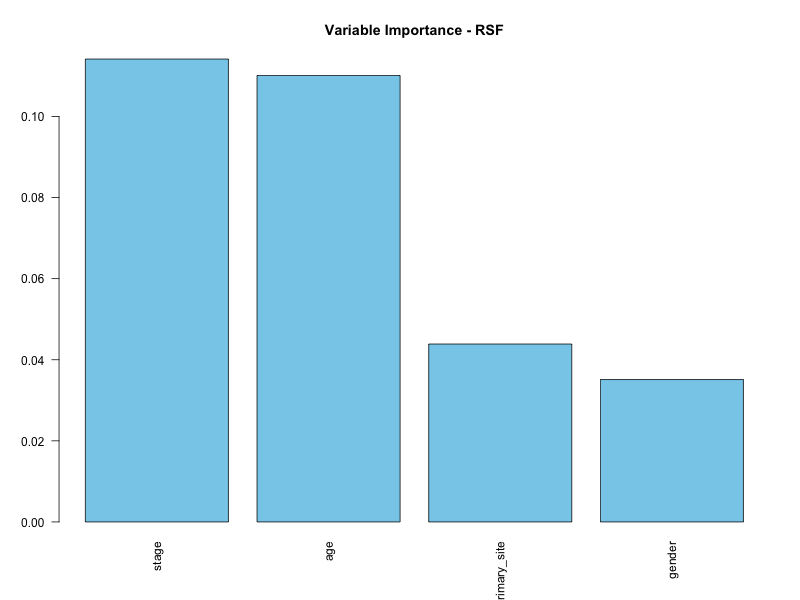
\includegraphics[width=0.8\linewidth]{../outputs/plots/rsf/rsf_variable_importance}

\subsection{Penalized Cox (CoxNet)}\label{penalized-cox-coxnet}

\begin{Shaded}
\begin{Highlighting}[]
\FunctionTok{print}\NormalTok{(}\FunctionTok{coef}\NormalTok{(cv\_cox, }\AttributeTok{s =} \StringTok{"lambda.min"}\NormalTok{))}
\end{Highlighting}
\end{Shaded}

\begin{verbatim}
## 12 x 1 sparse Matrix of class "dgCMatrix"
##                                   1
## age                      0.01909276
## genderMale              -0.06109987
## stageStage II            .         
## stageStage III           0.06727412
## stageStage IVA           0.67042557
## stageStage IVB           1.25936624
## stageStage IVC           3.15305937
## primary_siteLarynx      -0.48072775
## primary_siteOral Cavity  .         
## primary_siteOral Tongue  .         
## primary_siteTonsil      -0.42467144
## primary_siteOther       -0.20556011
\end{verbatim}

\begin{Shaded}
\begin{Highlighting}[]
\NormalTok{knitr}\SpecialCharTok{::}\FunctionTok{include\_graphics}\NormalTok{(}\FunctionTok{here}\NormalTok{(}\StringTok{"outputs"}\NormalTok{, }\StringTok{"plots"}\NormalTok{, }\StringTok{"survival"}\NormalTok{, }\StringTok{"coxnet\_variable\_importance.png"}\NormalTok{))}
\end{Highlighting}
\end{Shaded}

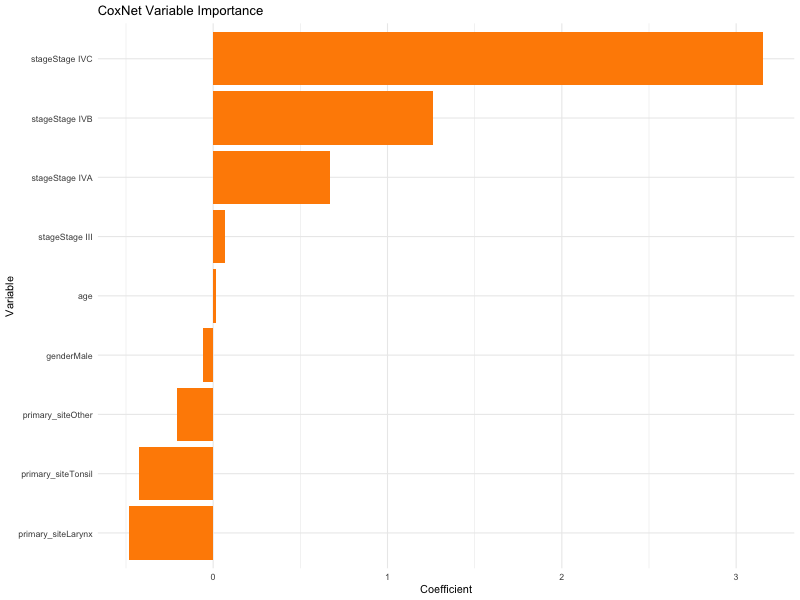
\includegraphics[width=0.8\linewidth]{../outputs/plots/survival/coxnet_variable_importance}

\begin{Shaded}
\begin{Highlighting}[]
\NormalTok{knitr}\SpecialCharTok{::}\FunctionTok{include\_graphics}\NormalTok{(}\FunctionTok{here}\NormalTok{(}\StringTok{"outputs"}\NormalTok{, }\StringTok{"plots"}\NormalTok{, }\StringTok{"survival"}\NormalTok{, }\StringTok{"coxnet\_cv\_curve.png"}\NormalTok{))}
\end{Highlighting}
\end{Shaded}

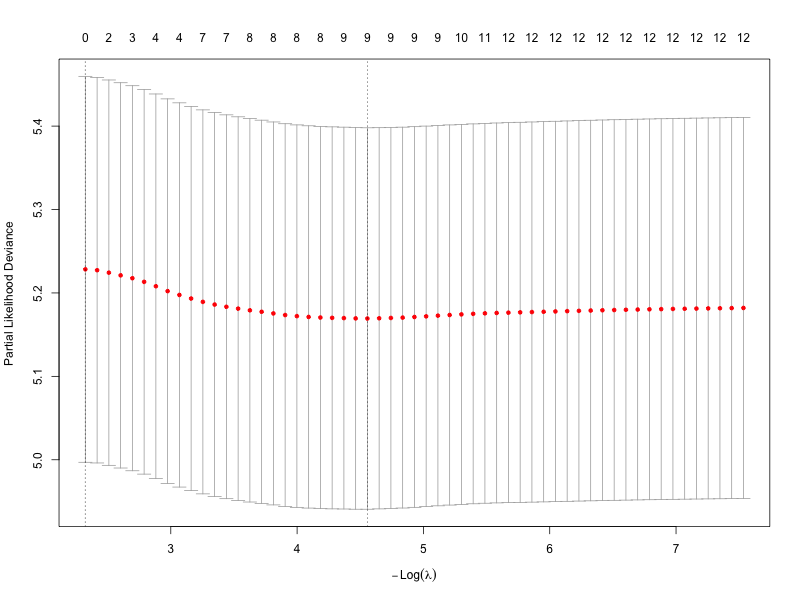
\includegraphics[width=0.8\linewidth]{../outputs/plots/survival/coxnet_cv_curve}

\section{7. Subgroup Survival
Estimates}\label{subgroup-survival-estimates}

\begin{Shaded}
\begin{Highlighting}[]
\NormalTok{subgroup\_table }\OtherTok{\textless{}{-}} \FunctionTok{read\_csv}\NormalTok{(}\FunctionTok{here}\NormalTok{(}\StringTok{"outputs"}\NormalTok{, }\StringTok{"tables"}\NormalTok{,}\StringTok{"coxnet\_subgroup\_medians.csv"}\NormalTok{))}
\NormalTok{knitr}\SpecialCharTok{::}\FunctionTok{kable}\NormalTok{(subgroup\_table, }\AttributeTok{caption =} \StringTok{"Median Survival by Subgroup (CoxNet)"}\NormalTok{)}
\end{Highlighting}
\end{Shaded}

\begin{longtable}[]{@{}lr@{}}
\caption{Median Survival by Subgroup (CoxNet)}\tabularnewline
\toprule\noalign{}
Group & Median\_Survival\_Months \\
\midrule\noalign{}
\endfirsthead
\toprule\noalign{}
Group & Median\_Survival\_Months \\
\midrule\noalign{}
\endhead
\bottomrule\noalign{}
\endlastfoot
Age 50 & 109.970 \\
Age 60 & 90.755 \\
Age 70 & 74.950 \\
Male & 90.755 \\
Female & 87.780 \\
\end{longtable}

\begin{Shaded}
\begin{Highlighting}[]
\NormalTok{knitr}\SpecialCharTok{::}\FunctionTok{include\_graphics}\NormalTok{(}\FunctionTok{here}\NormalTok{(}\StringTok{"outputs"}\NormalTok{, }\StringTok{"plots"}\NormalTok{, }\StringTok{"survival"}\NormalTok{,}\StringTok{"coxnet\_predicted\_survival\_age.png"}\NormalTok{))}
\end{Highlighting}
\end{Shaded}

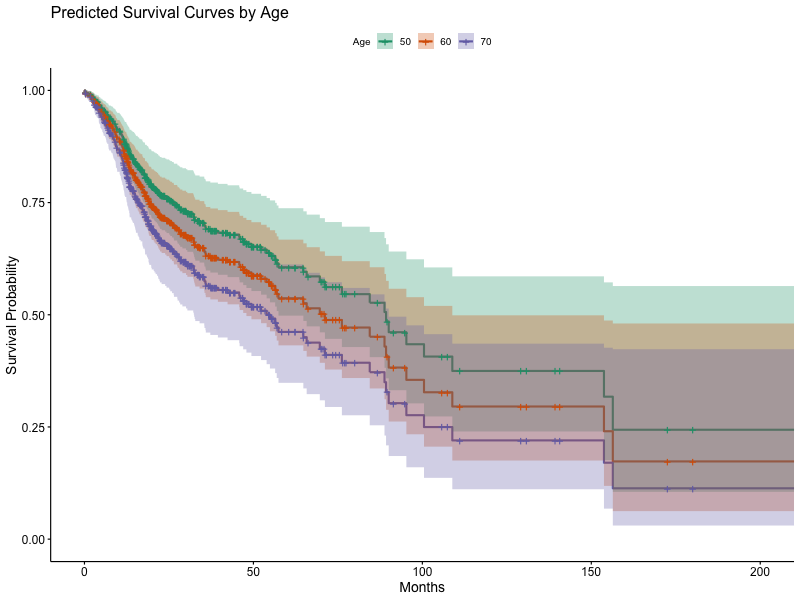
\includegraphics[width=0.8\linewidth]{../outputs/plots/survival/coxnet_predicted_survival_age}

\begin{Shaded}
\begin{Highlighting}[]
\NormalTok{knitr}\SpecialCharTok{::}\FunctionTok{include\_graphics}\NormalTok{(}\FunctionTok{here}\NormalTok{(}\StringTok{"outputs"}\NormalTok{, }\StringTok{"plots"}\NormalTok{, }\StringTok{"survival"}\NormalTok{, }\StringTok{"coxnet\_predicted\_survival\_gender.png"}\NormalTok{))}
\end{Highlighting}
\end{Shaded}

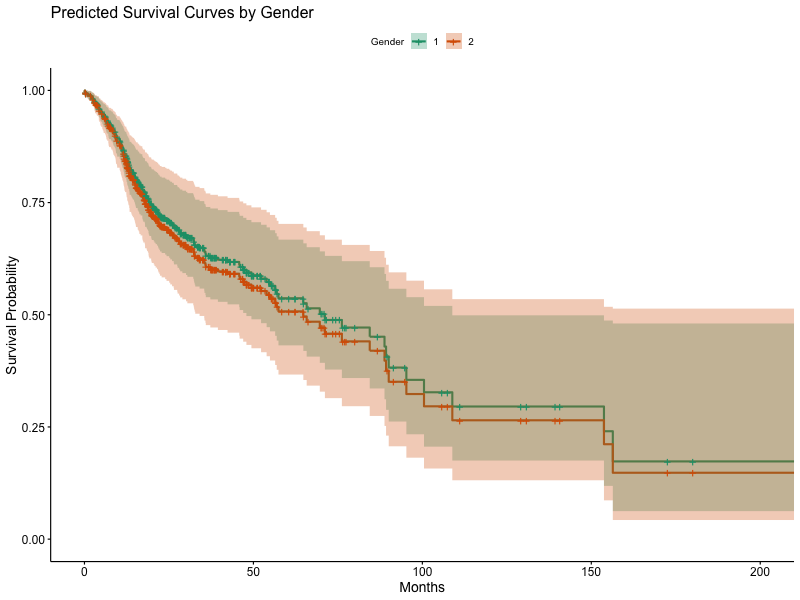
\includegraphics[width=0.8\linewidth]{../outputs/plots/survival/coxnet_predicted_survival_gender}

\section{8. Model Performance
Comparison}\label{model-performance-comparison}

\begin{Shaded}
\begin{Highlighting}[]
\NormalTok{model\_results }\OtherTok{\textless{}{-}} \FunctionTok{read\_csv}\NormalTok{(}\FunctionTok{here}\NormalTok{(}\StringTok{"outputs"}\NormalTok{, }\StringTok{"tables"}\NormalTok{, }\StringTok{"final\_model\_performance\_summary.csv"}\NormalTok{))}
\end{Highlighting}
\end{Shaded}

\begin{Shaded}
\begin{Highlighting}[]
\NormalTok{knitr}\SpecialCharTok{::}\FunctionTok{include\_graphics}\NormalTok{(}\FunctionTok{here}\NormalTok{(}\StringTok{"outputs"}\NormalTok{, }\StringTok{"plots"}\NormalTok{, }\StringTok{"final\_model\_comparison\_plot.png"}\NormalTok{))}
\end{Highlighting}
\end{Shaded}

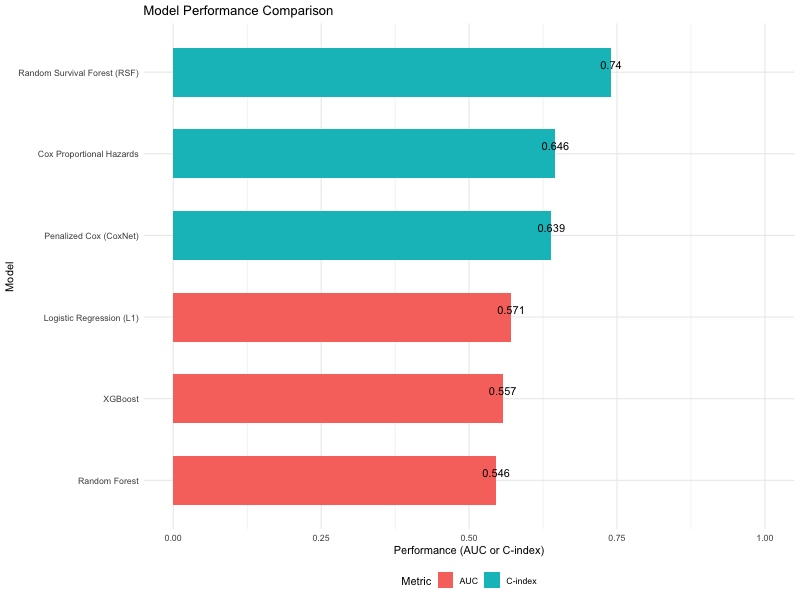
\includegraphics[width=0.8\linewidth]{../outputs/plots/final_model_comparison_plot}

\section{9. Interpretation}\label{interpretation}

\begin{itemize}
\tightlist
\item
  The best performing model was Random Survival Forest (C-index = 0.74),
  suggesting strong potential for modeling censored survival outcomes
  using ensemble methods.
\item
  Penalized Cox regression (C-index = 0.639) also showed good
  discrimination, with regularization helping to focus on relevant
  predictors.
\item
  Classification-based ML models (RF, XGBoost, logistic) showed lower
  AUCs, potentially due to class imbalance and loss of time-to-event
  granularity.
\end{itemize}

\section{10. Conclusion}\label{conclusion}

This project demonstrates that:

\begin{itemize}
\tightlist
\item
  Time-to-event models are more appropriate than binary classifiers in
  survival analysis contexts.
\item
  RSF models are effective for clinical survival prediction.
\item
  Regularized Cox models like CoxNet strike a balance between
  performance and interpretability.
\item
  The analysis pipeline here provides a template for applying survival
  ML methods to other clinical or public health prediction tasks.
\end{itemize}

\begin{center}\rule{0.5\linewidth}{0.5pt}\end{center}

\end{document}
